% !TeX program = xelatex
\documentclass[11pt,a4paper]{article}

\usepackage[a4paper,top=24mm,bottom=23mm,left=25mm,right=25mm,headheight=22pt]{geometry}
\usepackage{fontspec}
\defaultfontfeatures{Ligatures=TeX,Scale=MatchLowercase}
\IfFontExistsTF{Times New Roman}{
  \setmainfont{Times New Roman}
}{
  % Portable metric-compatible fallback for non-Windows build systems.
  \setmainfont{TeX Gyre Termes}
}
\usepackage{microtype}
\usepackage{setspace}
\setstretch{1.08}
\usepackage{graphicx}
\graphicspath{{../figures/}}
\usepackage{booktabs,longtable,tabularx,array,multirow}
\usepackage{adjustbox}
\usepackage{pdflscape}
\usepackage{caption}
\usepackage{float}
\usepackage[section]{placeins}
\usepackage{enumitem}
\usepackage[table]{xcolor}
\usepackage{titlesec}
\usepackage{fancyhdr}
\usepackage[numbers,sort&compress]{natbib}
\usepackage{url}
\usepackage[hidelinks,bookmarksnumbered,pdfencoding=auto]{hyperref}

\definecolor{navy}{HTML}{173B57}
\definecolor{teal}{HTML}{247A86}
\definecolor{lightblue}{HTML}{EAF2F6}
\definecolor{linegray}{HTML}{A9BBC7}
\definecolor{textgray}{HTML}{465862}
\hypersetup{
  pdftitle={Organoid Transplantation Research Landscape and Translational Applications},
  pdfauthor={Tharuniya Anpalakan},
  pdfsubject={Computational evidence mapping of organoid transplantation},
  pdfkeywords={organoid transplantation, evidence mapping, regenerative medicine, network analysis}
}

\titleformat{\section}{\Large\bfseries\color{navy}}{\thesection}{0.7em}{}
\titleformat{\subsection}{\large\bfseries\color{navy}}{\thesubsection}{0.6em}{}
\titleformat{\subsubsection}{\normalsize\bfseries\color{textgray}}{\thesubsubsection}{0.5em}{}
\titlespacing*{\section}{0pt}{18pt plus 3pt minus 2pt}{8pt}
\titlespacing*{\subsection}{0pt}{13pt plus 2pt minus 1pt}{5pt}

\captionsetup{font=small,labelfont={bf,color=navy},textfont={color=textgray},justification=justified,singlelinecheck=false,skip=7pt}
\captionsetup[table]{position=top}
\captionsetup[figure]{position=bottom}
\setcitestyle{numbers,square,comma,sort&compress}
\renewcommand{\bibsection}{\section*{References}\addcontentsline{toc}{section}{References}}
\renewcommand{\arraystretch}{1.18}
\setlist{itemsep=2pt,topsep=4pt,leftmargin=1.6em}
\newcolumntype{Y}{>{\raggedright\arraybackslash}X}
\newcolumntype{P}[1]{>{\raggedright\arraybackslash}p{#1}}

\pagestyle{fancy}
\fancyhf{}
\fancyhead[L]{\small\color{textgray}Organoid transplantation evidence map}
\fancyhead[R]{\small\color{textgray}Tharuniya Anpalakan}
\fancyfoot[C]{\small\color{textgray}\thepage}
\renewcommand{\headrulewidth}{0.4pt}
\renewcommand{\headrule}{\hbox to\headwidth{\color{linegray}\leaders\hrule height \headrulewidth\hfill}}

\begin{document}

\begin{titlepage}
  \thispagestyle{empty}
  \vspace*{22mm}
  \noindent{\color{teal}\rule{\textwidth}{2.2pt}}\\[16mm]
  \begin{center}
    {\fontsize{24}{30}\selectfont\bfseries\color{navy}
    Organoid Transplantation Research\\[1.5mm]
    Landscape and Translational Applications\par}
  \end{center}

  \vspace{12mm}
  \begin{center}
    \begin{minipage}{0.82\textwidth}
      \fontsize{14}{20}\selectfont\color{textgray}\hyphenpenalty=10000\exhyphenpenalty=10000
      A reproducible computational evidence-mapping study of engraftment, regenerative medicine and translational readiness
    \end{minipage}
  \end{center}

  \vspace{28mm}
  \begin{center}
    {\large\bfseries Tharuniya Anpalakan\par}
    \vspace{5mm}
    {\normalsize
    Department of Applied Sciences\\
    Northumbria University\\
    Newcastle upon Tyne, United Kingdom\\[3mm]
    \href{mailto:w25070895@northumbria.ac.lk}{w25070895@northumbria.ac.lk}\par}
  \end{center}

  \vfill
  \noindent{\color{teal}\rule{\textwidth}{2.2pt}}
\end{titlepage}

\pagenumbering{roman}

\section*{Abstract}
\addcontentsline{toc}{section}{Abstract}
Organoid transplantation has become an important experimental bridge between three-dimensional culture and regenerative medicine, but the evidence is fragmented across tissues, stem-cell sources, host species, graft sites and outcome definitions. This study developed a reproducible evidence map of 15 identifier-verified primary in vivo reports published from 2012 to 2023. Records were coded for organoid category, cell source, recipient model, graft location, engraftment, vascularization, functional outcome, safety reporting and translational limitations. A Python workflow checked identifiers and controlled vocabularies, generated descriptive summaries, constructed a study-provenanced heterogeneous research network and produced a descriptive translational evidence matrix. The final graph contained 64 nodes and 75 evidence-backed relationships. Kidney models formed the largest category (5/15), followed by intestinal (3/15) and retinal (3/15) constructs; all studies were preclinical. Fourteen reports described positive engraftment and one described failure to engraft at the intended injured-colon site. Vascularization was reported positively in ten studies and was not assessed in five. The biological endpoints were too heterogeneous for pooled efficacy analysis, ranging from epithelial repair and metabolic activity to glomerular tracer handling, visual responses and neural circuit interaction. No eligible human organoid-graft outcome study was present in the bounded corpus. The evidence supports organ-specific proof of concept, while manufacturing control, immune compatibility, physiological drainage or connectivity, prospective safety and long-term organ-scale function remain central translational barriers.

\noindent\textbf{Keywords:} organoids; transplantation; stem cells; regenerative medicine; evidence mapping; network analysis; translational research

\tableofcontents
\listoffigures
\listoftables
\clearpage
\pagenumbering{arabic}

\section{Introduction}

Organoids are three-dimensional, self-organizing cellular systems that reproduce selected structural or functional features of an organ. Their emergence from adult stem cells and pluripotent stem cells has enabled experimental access to human developmental programmes, tissue homeostasis and disease mechanisms that are incompletely represented by conventional monolayer cultures \citep{sato2009,spence2011,lancaster2013,clevers2016,rossi2018,kim2020}. Organoids are nevertheless models, not miniature organs in the complete physiological sense. They commonly lack mature vasculature, innervation, immune components, stromal diversity, mechanical loading, organ-scale geometry and routes for secretion or drainage \citep{jensen2023,hofer2021}.

Transplantation offers one route to overcome part of this limitation. A host can supply perfusion, extracellular matrix, endocrine signals and biomechanical cues, and can expose a construct to an injured or disease-relevant environment. These influences may promote survival, maturation and integration. They also introduce new sources of uncertainty: vascular structures may be host-derived, grafts may occupy ectopic sites, xenogeneic recipients may be immunodeficient, and an observed local function may not translate into replacement of whole-organ physiology. Recent engineering reviews consequently treat vascular access, defined biomaterials, immune compatibility, anatomical connection and scalable manufacture as linked design requirements rather than independent technical details \citep{brassard2019,park2024}. The scientific question is therefore not simply whether an organoid survives after implantation, but what biological process is demonstrated, under which conditions, for how long, and with what evidence of safety.

The organoid transplantation literature is especially difficult to compare because tissues demand different endpoints. Durable epithelial coverage can be meaningful in colon injury, whereas a kidney graft requires filtration together with urinary outflow, and a neural graft requires careful interpretation of electrophysiological integration and circuit consequences. A single numerical ``readiness score'' would compress these differences and risk implying a level of clinical comparability that the literature does not support.

This report presents a focused computational evidence map. Its centrepieces are a curated study database, a provenance-bearing research network and a descriptive translational evidence matrix. The work is designed to make the evidence traceable rather than to produce a pooled treatment effect. It extends earlier narrative work in this topic area while preserving the historical authorship of that separate publication \citep{sandamini2025}.

\subsection{Research questions}

The analysis addressed five questions:

\begin{enumerate}
  \item Which organoid categories, stem-cell sources and experimental models occur in the verified corpus?
  \item What forms of engraftment, vascular integration and tissue-specific function are reported?
  \item How are studies connected through shared biological and translational attributes?
  \item Which evidence domains are supported, uncertain or unassessed within each organoid category?
  \item Which barriers most clearly separate animal proof of concept from responsible human translation?
\end{enumerate}

\section{Scientific background}

\subsection{Organoid identity and model boundaries}

Self-organization is central to organoid biology. Adult tissue-derived systems often retain the epithelial identity and renewal programme of the source tissue, as illustrated by long-term intestinal crypt--villus cultures initiated from Lgr5-positive stem cells \citep{sato2009}. Pluripotent stem-cell systems use staged developmental signalling to generate tissues such as intestine, brain and kidney \citep{spence2011,lancaster2013,takasato2015,morizane2015}. Engineered co-culture and spatial control can add complexity, but greater complexity does not by itself establish physiological completeness \citep{takebe2019,hofer2021}. Contemporary consensus papers also emphasize that naming should reflect the source, tissue identity, developmental scope and degree of organization rather than imply that a construct is a complete organ \citep{marsee2021,pasca2022,jensen2023}.

For this map, an organoid was distinguished from four neighbouring concepts (Table~\ref{tab:boundaries}). This distinction matters because transplantation of isolated cells, an epithelial monolayer or a whole donor organ answers a different question from transplantation of a self-organized three-dimensional construct.

\begin{table}[H]
\centering
\caption{Operational boundaries used to distinguish organoid transplantation from related interventions.}
\label{tab:boundaries}
\begin{tabularx}{\textwidth}{@{}P{28mm}YY@{}}
\toprule
\textbf{Construct} & \textbf{Defining feature} & \textbf{Treatment in this evidence map}\\
\midrule
Organoid or organ bud & Self-organizing 3D tissue with organ-associated lineages or architecture & Eligible when transplanted into a living recipient and evaluated in vivo\\
Organoid-derived sheet & Organized 3D tissue sheet produced through an organoid differentiation process & Eligible when the transplanted unit retained a tissue-level organization\\
Spheroid & Cell aggregate that may lack organ-specific organization & Excluded unless the source study established an organoid or organ-bud identity\\
Isolated-cell therapy & Dissociated cells or a purified monolayer & Excluded from the analytic corpus\\
Whole-organ transplant & Anatomically complete donor organ with established clinical terminology & Excluded; outside the biological scope of organoid transplantation\\
\bottomrule
\end{tabularx}
\end{table}

\subsection{Stem-cell sources and product characteristics}

Adult stem-cell organoids can preserve donor- and tissue-specific epithelial characteristics and support long-term expansion. Their lineage range may be narrower, and missing stromal or immune components often need deliberate reconstruction. Pluripotent stem cells---embryonic stem cells (ESCs) and induced pluripotent stem cells (iPSCs)---permit differentiation across germ layers and therefore enable complex developmental models. Their translational use requires control of line-to-line variation, residual pluripotency, off-target populations, genomic stability and manufacturing consistency \citep{bartfeld2017,rossi2018,kim2020,jensen2023}. Long-term expansion studies in liver illustrate both the regenerative opportunity and the importance of genomic quality control \citep{huch2015}. Engineering strategies can improve reproducibility and geometry, but the added materials, devices and cell populations must themselves be defined and qualified for clinical manufacture \citep{brassard2019,park2024}.

The distinction between derivation and transplantation is also important. Foundational protocols establish that a construct can be made reproducibly in vitro \citep{spence2011,takasato2015,morizane2015}; transplantation studies then ask whether it survives, integrates or matures in a host. Both bodies of work inform translation, but only the latter were counted in the analytic cohort.

\subsection{Tissue-specific translational logic}

\subsubsection{Intestinal and colonic constructs}

Intestinal organoids have strong biological grounding in adult stem-cell culture and directed differentiation. After transplantation, meaningful endpoints include epithelial coverage, lineage differentiation, barrier properties and durable renewal. Location is decisive: ectopic sites may support growth and maturation without demonstrating repair at the intended intestinal lesion. This distinction is visible in the mapped evidence, in which one study reported positive ectopic outcomes but negative engraftment at the injured colon.

\subsubsection{Liver organ buds}

Liver organ-bud strategies seek rapid vascular connection and metabolic contribution. Protein secretion or drug-metabolism measurements provide useful functional evidence, but small ectopic grafts do not reproduce liver mass, biliary drainage, zonation or the full metabolic reserve of the native organ. Evidence should therefore be framed as partial tissue function rather than organ replacement.

\subsubsection{Kidney organoids}

Kidney organoids contain segmented nephron-like structures and can reproduce aspects of nephrogenesis and toxicity in vitro \citep{takasato2015,morizane2015}. Transplantation can promote glomerular and tubular maturation and host vascular ingrowth. Yet filtration in a subset of glomerular structures does not constitute renal replacement. A translational kidney graft would also require sufficient nephron mass, collecting-system connection, urinary drainage, endocrine regulation and stable host integration.

\subsubsection{Retinal tissue}

Retinal organoid sheets can provide a spatially organized photoreceptor source. Functional interpretation may combine histological integration, electrophysiology and visually guided behaviour, but degeneration models, surgical placement, rosette formation and off-target tissue risk all affect inference. Prospective tumorigenicity testing and standardized product identity are particularly important for pluripotent stem-cell-derived sheets.

\subsubsection{Brain and cortical organoids}

Cerebral organoids originated as developmental models with region-like organization \citep{lancaster2013}. After grafting, vascularization and electrophysiological interaction with host circuits can provide evidence of maturation. These observations are scientifically important but do not themselves define a therapeutic benefit. Neural transplantation also raises distinctive questions about circuit-level effects, animal welfare and the ethical oversight of human--animal neural chimerism. Responsible translation must be consistent with rigorous stem-cell research and clinical standards \citep{lovellbadge2021}.

\section{Methods}

\subsection{Study design}

The project was designed as a structured evidence map rather than an exhaustive systematic review. It combines manual literature curation with deterministic computational validation and descriptive analysis. The unit of analysis is a primary report of an organoid, organ bud or organoid-derived tissue sheet transplanted into a living recipient. Reporting concepts were informed by the PRISMA extension for scoping reviews, although this bounded, single-reviewer map is not presented as a PRISMA-compliant systematic review \citep{tricco2018}. The workflow is summarized in Figure~\ref{fig:workflow}.

\begin{figure}[H]
\centering
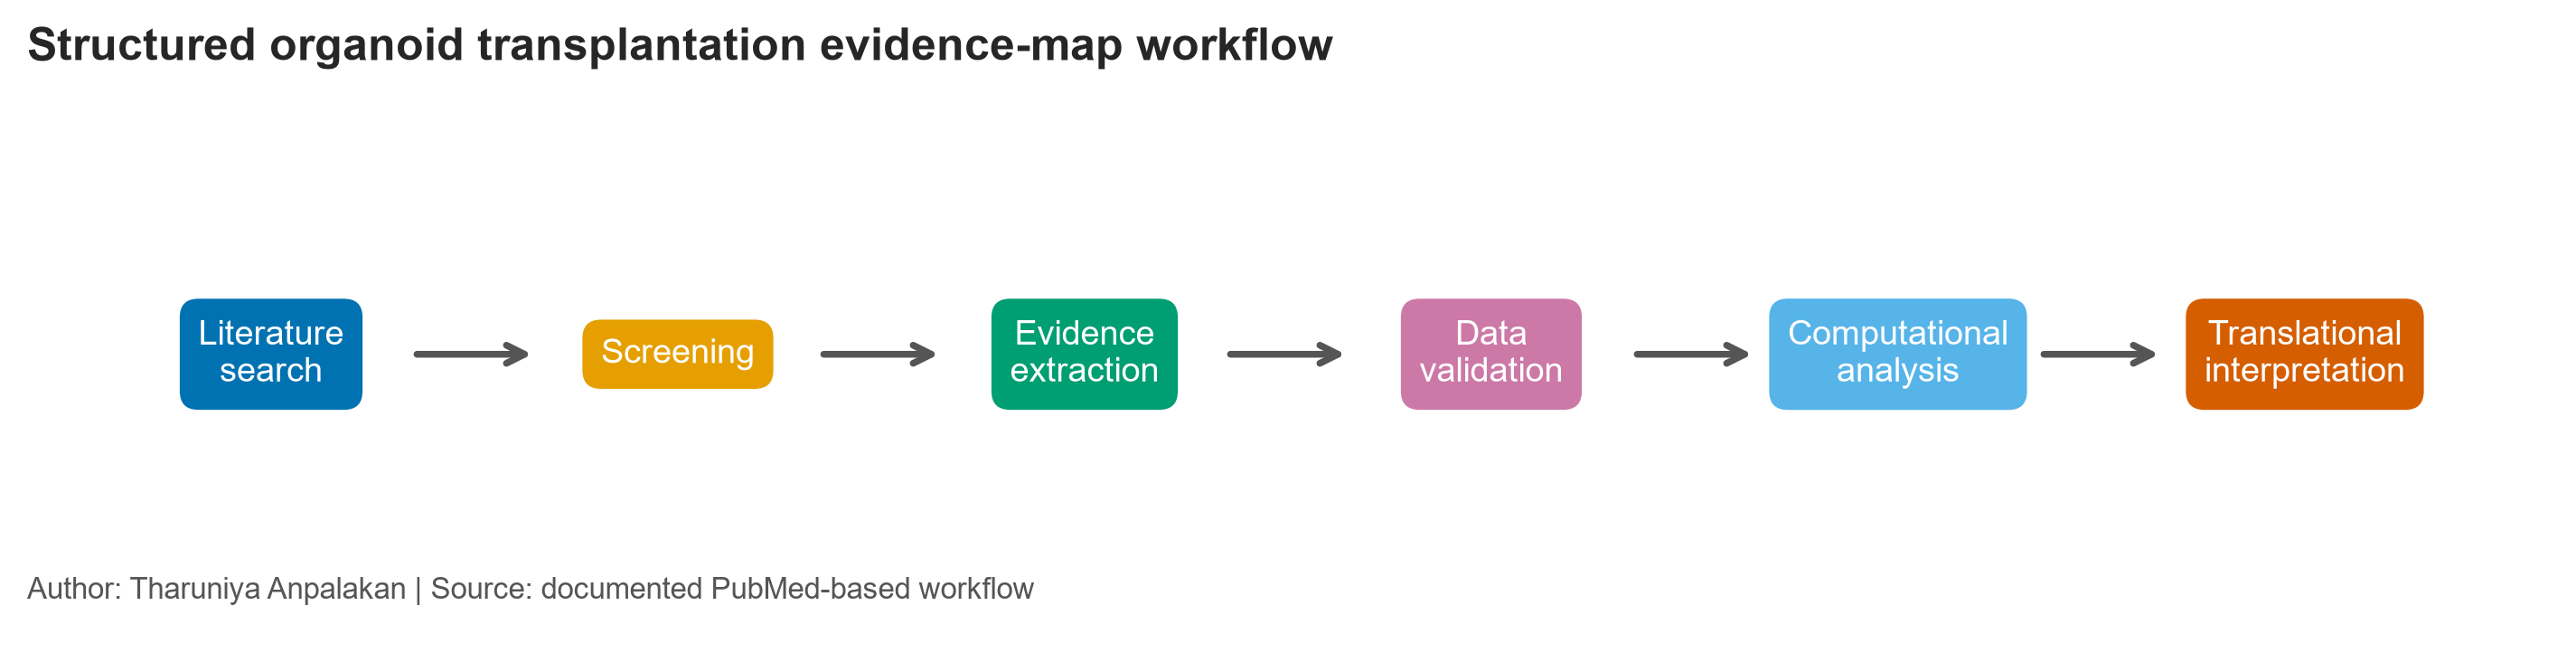
\includegraphics[width=0.96\textwidth]{figure_01_research_workflow.png}
\caption{Reproducible evidence-mapping workflow. Literature records were screened against explicit biological boundaries, converted to a structured dataset, validated, analysed and interpreted without converting record frequency into therapeutic efficacy.}
\label{fig:workflow}
\end{figure}

\subsection{Literature acquisition}

PubMed searches were performed on 18 October 2026 using combinations of \texttt{organoid*}, \texttt{transplant*}, \texttt{engraft*} and organ-specific terms. Backward checking from the supplied research materials was used to identify seminal reports. PubMed identifier pages were used to verify titles, journals, years, DOIs and PMIDs. ClinicalTrials.gov was consulted only to clarify the distinction between preclinical evidence and human clinical investigation; registry records without peer-reviewed organoid-graft outcomes were not eligible.

The search was intentionally bounded. It was designed to establish a reliable seed corpus and computational framework, not to claim exhaustive coverage of every database or language. The repository records exact queries, retrieval date and source links in \path{docs/search_strategy.md} and \path{data/metadata/search_log.csv}.

\subsection{Eligibility criteria}

\begin{table}[H]
\centering
\caption{Eligibility criteria applied during study selection.}
\label{tab:eligibility}
\begin{tabularx}{\textwidth}{@{}P{27mm}YY@{}}
\toprule
\textbf{Domain} & \textbf{Included} & \textbf{Excluded}\\
\midrule
Publication & Primary research with a traceable bibliographic record & Reviews, editorials, protocols without transplant outcomes and announcements\\
Construct & Organoid, organ bud or organoid-derived organized 3D tissue sheet & Conventional cell suspensions, simple spheroids without organoid evidence, fetal tissue and whole organs\\
Intervention & Implantation into a living animal or human recipient & In vitro culture only, ex vivo perfusion only or computational simulation only\\
Outcome & In vivo survival, engraftment, vascularization, maturation, function or safety & Reports without post-transplant evaluation\\
Evidence stage & Preclinical or clinical outcome evidence & Registry entries without reported outcomes\\
\bottomrule
\end{tabularx}
\end{table}

\subsection{Data extraction and coding}

Twenty-three fields were retained for each report, including study identifier, citation, DOI, PMID, organoid category, stem-cell source, target tissue, disease context, recipient model, graft site, transplantation approach, evidence stage, engraftment, vascularization, functional outcome, safety, limitations, design and direct source link. Categorical outcomes used five states: \emph{reported positive}, \emph{reported negative}, \emph{not assessed}, \emph{not reported} and \emph{unclear}. This vocabulary prevents missing information from being recoded as biological failure.

The evidence-quality table records whether an experimental model and control design are identifiable, whether engraftment and functional outcomes were assessed, whether safety was examined and how directly the work informs clinical application. It does not assign a universal composite score, because validity criteria differ substantially among retinal, renal, intestinal and neural experiments.

Because every included transplantation experiment used an animal recipient, interpretation also considered the reporting domains emphasized by ARRIVE 2.0: study design, sample-size justification, inclusion and exclusion criteria, randomization, blinding, outcome definition and statistical methods \citep{perciedusert2020}. These items were not uniformly recoverable from the structured bibliographic corpus and were therefore treated as appraisal targets rather than assumed indicators of study quality.

\subsection{Validation and computational analysis}

The Python pipeline checks required columns, unique study IDs, DOI and PMID syntax, duplicated identifiers, controlled vocabularies and structural missingness. Descriptive counts were produced with pandas. NetworkX was used to construct an undirected heterogeneous graph linking organoid categories to cell sources, target tissues, experimental models, engraftment states and documented barriers. Every edge stores the supporting study IDs and an evidence count. The layout uses a fixed random seed of 42 for reproducibility.

The translational matrix aggregates categorical support across seven domains: in vitro functional characterization, preclinical engraftment, vascular integration, functional maturation, safety assessment, human clinical investigation, and manufacturing or scale-up. Matrix states are descriptive:

\begin{itemize}
  \item \textbf{Supported}: at least one included study documents the domain;
  \item \textbf{Unsupported}: an assessed negative result is present without positive support;
  \item \textbf{Uncertain}: evidence is incomplete, conditional or conflicting;
  \item \textbf{Unassessed}: the domain was not evaluated in the mapped corpus.
\end{itemize}

No meta-analysis was attempted. Outcome definitions, host species, graft sites, follow-up periods and biological purposes were too heterogeneous for a defensible pooled effect estimate.

\subsection{Translational assessment framework}

Clinical translation was interpreted as a chain of evidence rather than a single readiness score. Table~\ref{tab:translationframework} defines the domains used to separate biological proof of concept from product-development evidence. This distinction is consistent with contemporary organoid engineering, personalized-medicine and stem-cell translation literature \citep{lovellbadge2021,sotogamez2024,park2024,septiana2024}.

\begin{table}[H]
\centering
\small
\caption{Translational assessment domains used to interpret organoid-graft evidence. The domains are complementary; strength in one domain does not compensate for absent evidence in another.}
\label{tab:translationframework}
\begin{tabularx}{\textwidth}{@{}P{30mm}YY@{}}
\toprule
\textbf{Domain} & \textbf{Evidence sought} & \textbf{Reason for clinical relevance}\\
\midrule
Identity and purity & Defined cell populations, tissue architecture, off-target cells and residual pluripotency & Establishes what is implanted and constrains tumorigenic or ectopic-tissue risk\\
Potency & Quantitative assay linked to the proposed mechanism of action & Connects a release test to the intended biological effect\\
Manufacture & Batch consistency, genomic stability, scalable culture and clinically compatible matrix & Determines whether the product can be reproduced under controlled conditions\\
Delivery & Graft format, implantation route, anatomical retention and surgical feasibility & Links laboratory construct design to the target organ and procedure\\
Integration & Perfusion plus tissue-specific neural, ductal, luminal or collecting-system connection & Distinguishes local survival from physiologically useful incorporation\\
Immune compatibility & Allogeneic or autologous strategy, immunogenicity and host-response evidence & Determines rejection risk and the need for immunosuppression or immune engineering\\
Safety and durability & Biodistribution, overgrowth, tumorigenicity, ectopic tissue and long-term follow-up & Addresses delayed harms that short efficacy experiments may not detect\\
Clinical benefit & Patient-relevant outcome, comparator, durability and post-treatment surveillance & Demonstrates benefit beyond histological or surrogate evidence\\
\bottomrule
\end{tabularx}
\end{table}

\section{Results}

\subsection{Dataset characteristics}

Fifteen primary reports passed the eligibility and structural validation checks. They covered six organoid categories, five recorded stem-cell-source categories and nine experimental-model labels. Publication years ranged from 2012 to 2023. All 15 records contained a DOI and PMID, yielding 30 verified source identifiers. All eligible studies were preclinical in vivo investigations.

\begin{table}[H]
\centering
\caption{Verified corpus and analysis outputs. Counts refer to the bounded analytic dataset, not the entire organoid field.}
\label{tab:summary}
\begin{tabularx}{0.9\textwidth}{@{}Y>{\raggedleft\arraybackslash}P{28mm}@{}}
\toprule
\textbf{Measure} & \textbf{Result}\\
\midrule
Eligible primary studies & 15\\
Publication-year coverage & 2012--2023\\
Organoid categories & 6\\
Stem-cell-source categories & 5\\
Experimental-model labels & 9\\
Verified DOI identifiers & 15\\
Verified PMID identifiers & 15\\
Evidence stage & 15 preclinical in vivo\\
Research network & 64 nodes; 75 edges\\
Translational matrix & 6 organoid categories; 7 domains\\
\bottomrule
\end{tabularx}
\end{table}

The publication timeline is uneven (Figure~\ref{fig:timeline}) and should be understood as the chronology of this focused sample rather than a bibliometric estimate of the entire field.

\begin{figure}[H]
\centering
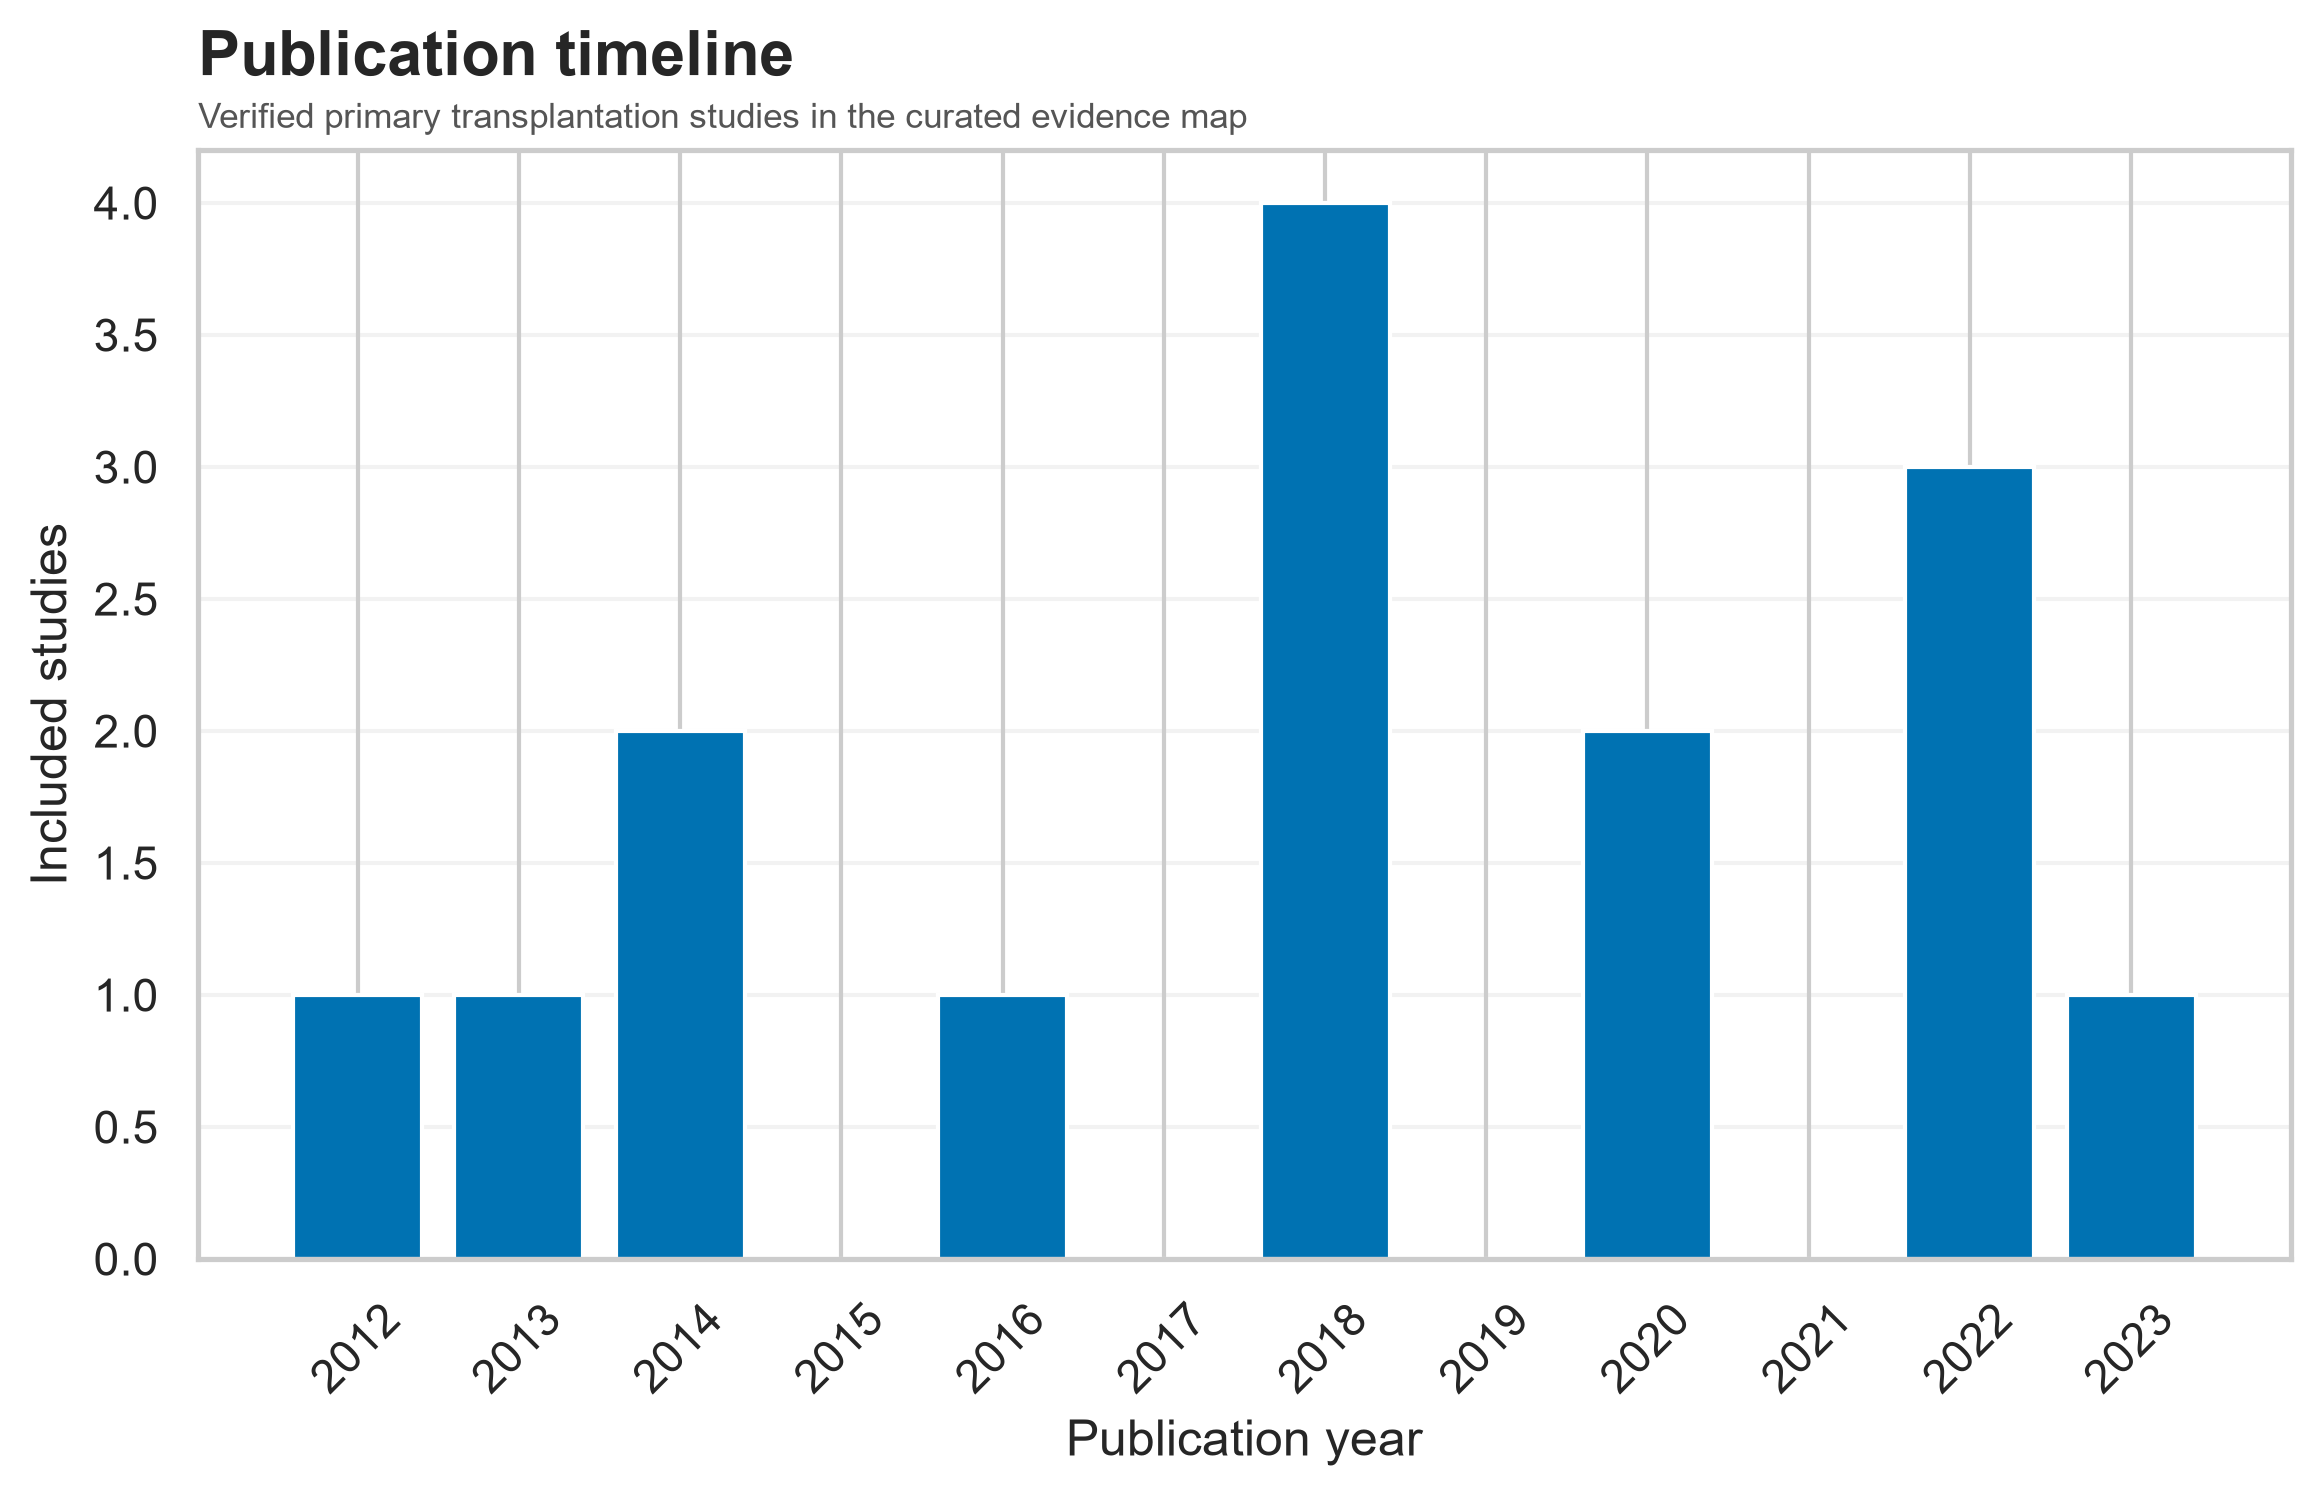
\includegraphics[width=0.88\textwidth]{figure_02_publication_timeline.png}
\caption{Publication timeline for the 15 included studies. Counts reflect eligible records in the curated corpus and are not a measure of research quality or therapeutic success.}
\label{fig:timeline}
\end{figure}

\subsection{Distribution by organoid type and cell source}

Kidney organoids were the most frequent category (5/15), followed by intestinal (3/15), retinal (3/15), brain (2/15), colonic (1/15) and liver (1/15) constructs (Figure~\ref{fig:orgdist}). This pattern reflects the search and inclusion framework as well as genuine experimental activity. It does not establish that kidney applications are more clinically advanced.

\begin{figure}[H]
\centering
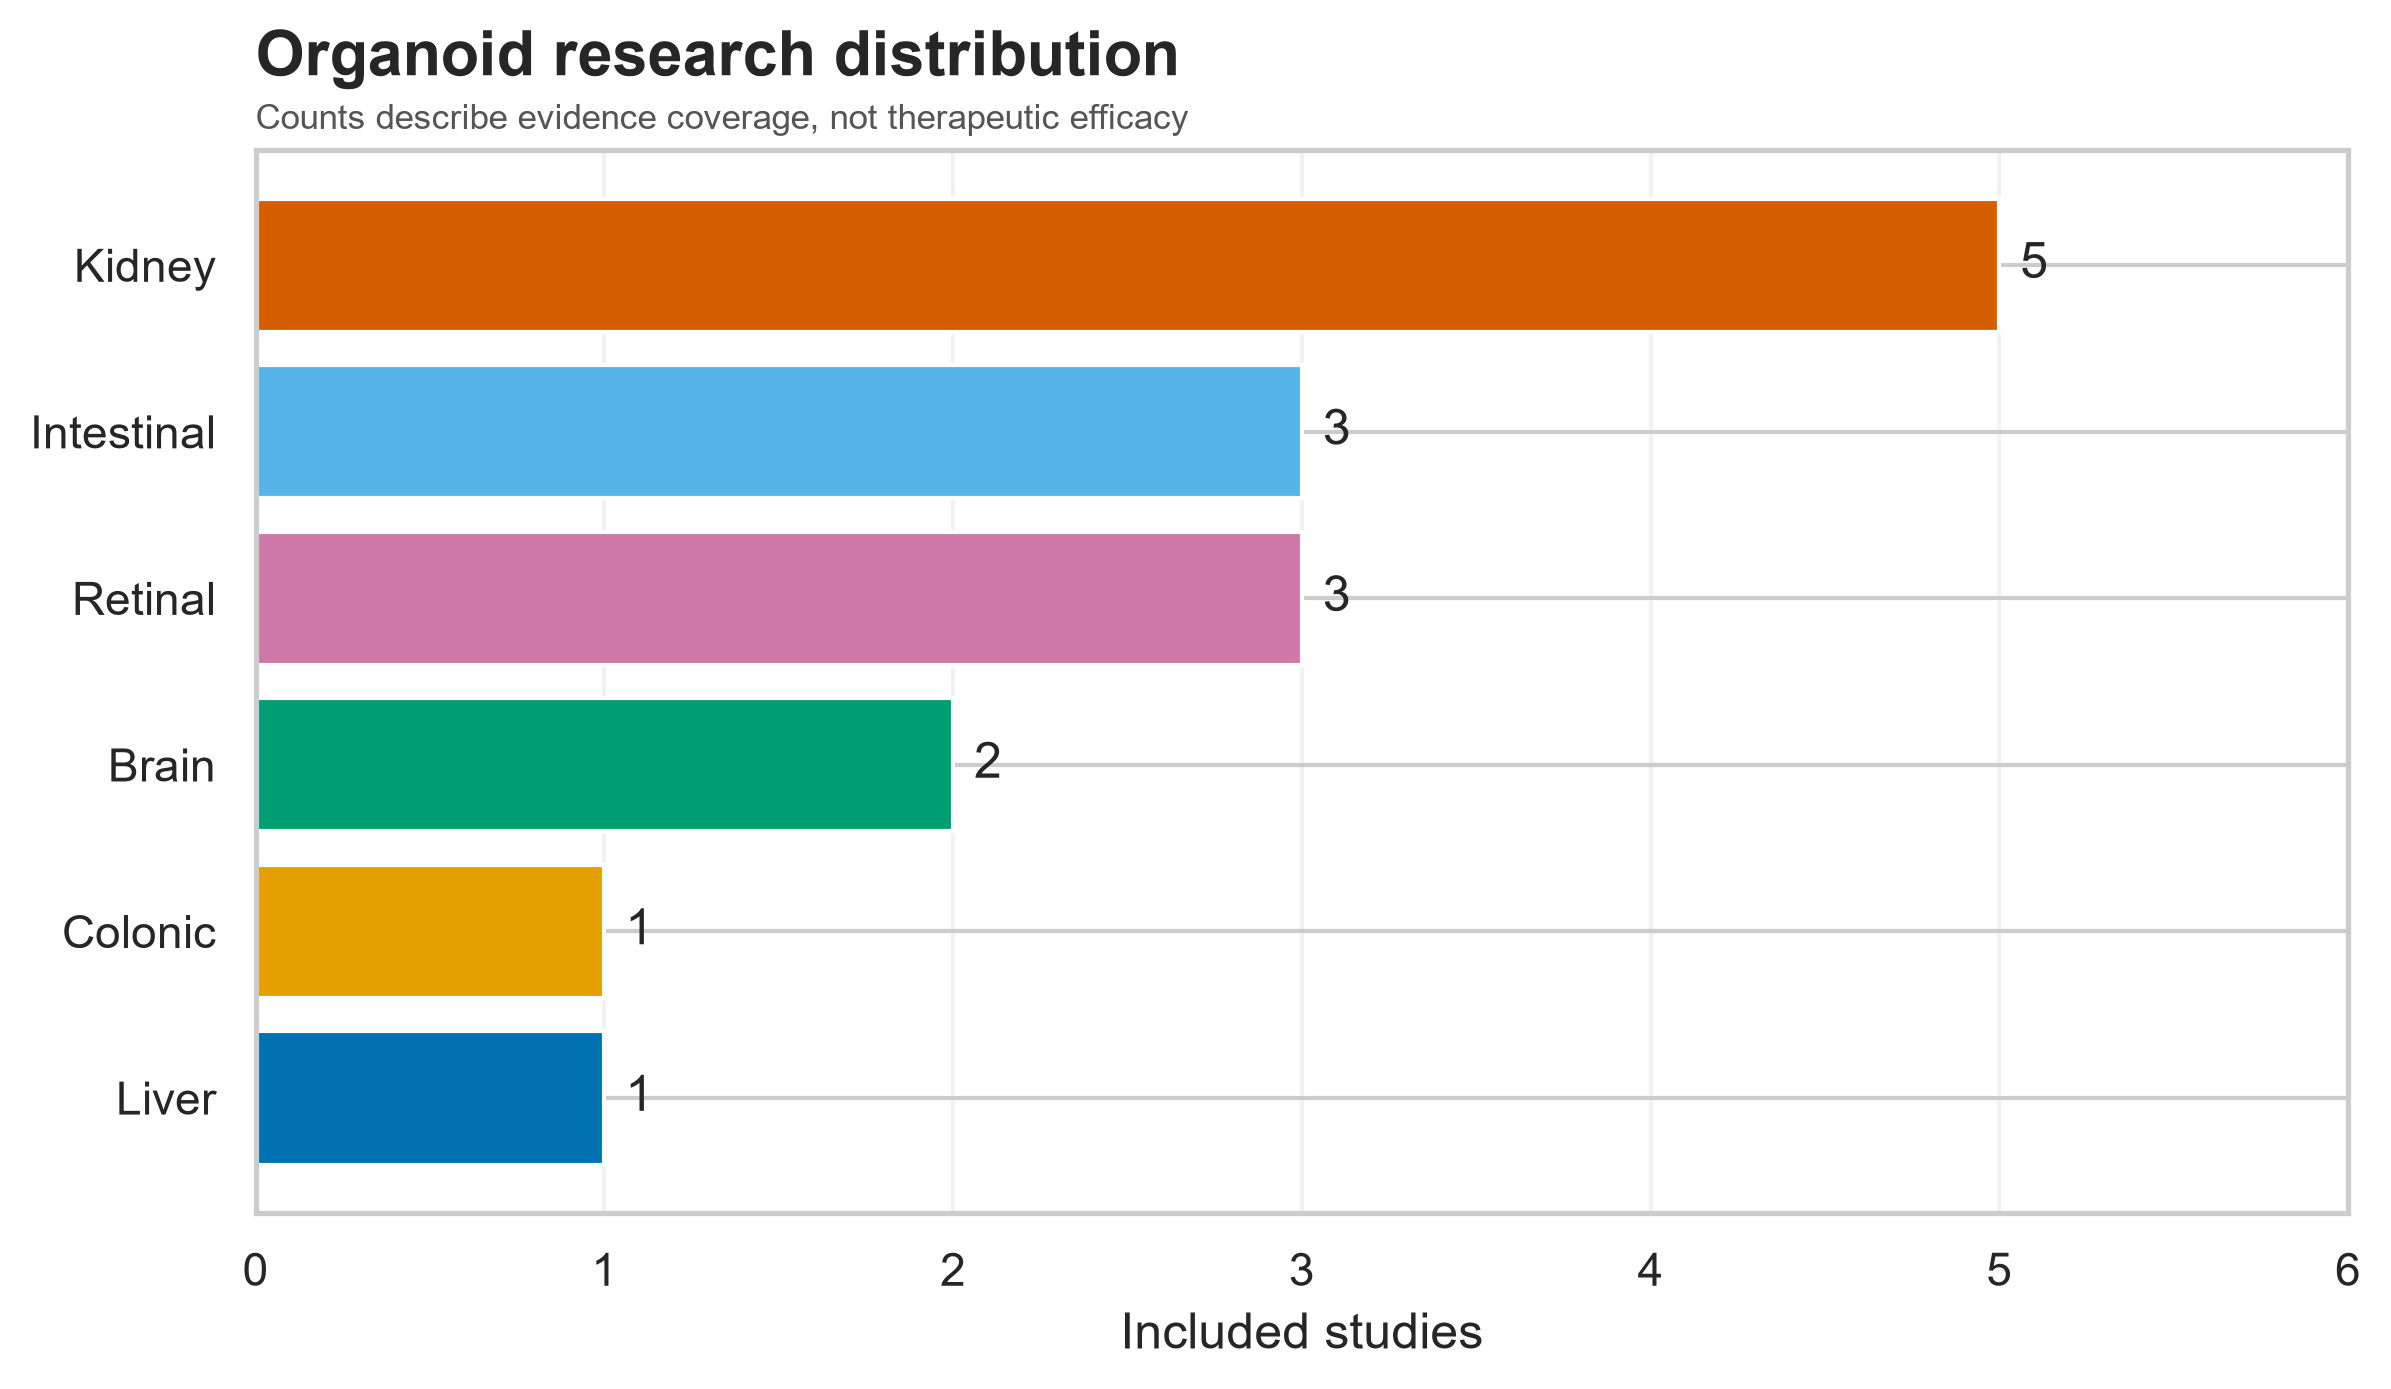
\includegraphics[width=0.88\textwidth]{figure_03_organoid_distribution.png}
\caption{Distribution of included studies by organoid category. The denominator is 15 studies; categories were assigned using the transplanted construct described in each report.}
\label{fig:orgdist}
\end{figure}

Induced pluripotent stem cells were the most common recorded source (7/15). Three reports used the broader designation human pluripotent stem cells, two combined embryonic and induced pluripotent stem-cell constructs, two used embryonic stem cells and one used adult stem cells (Figure~\ref{fig:cellsources}). These labels preserve the terminology supported by each source record rather than inferring a more specific cell line.

\begin{figure}[H]
\centering
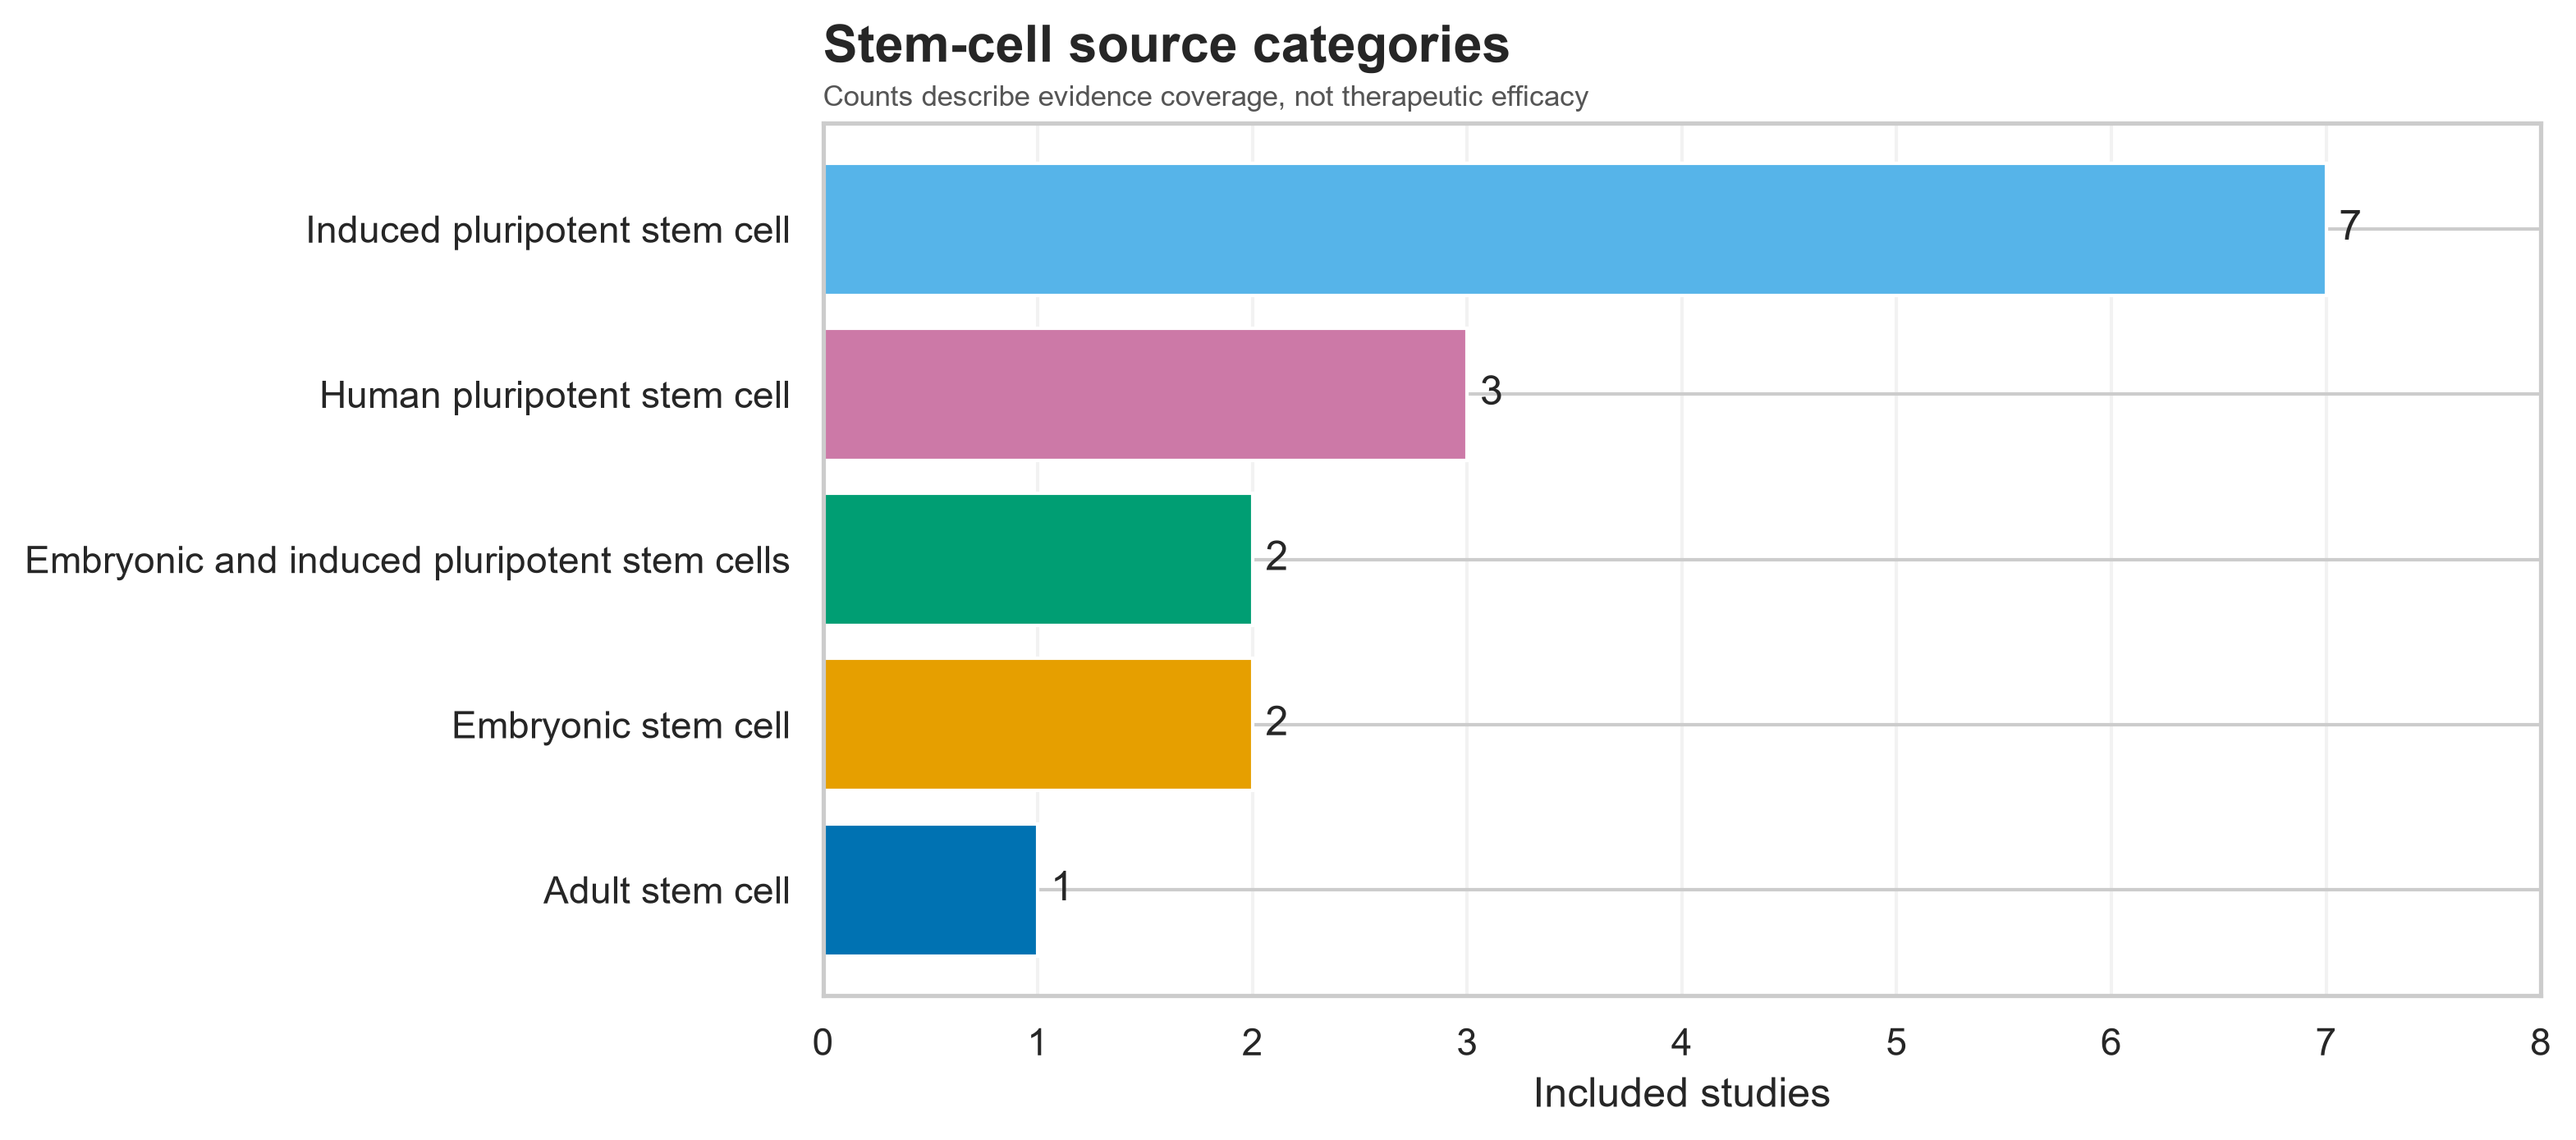
\includegraphics[width=0.90\textwidth]{figure_04_stem_cell_sources.png}
\caption{Stem-cell sources recorded in the curated database. The categories are mutually exclusive at study level and preserve source-report terminology.}
\label{fig:cellsources}
\end{figure}

\subsection{Study-level evidence inventory}

Table~\ref{tab:inventory} shows the analytic cohort and the principal interpretation attached to each report. The table is an evidence inventory, not a ranking.

\begin{landscape}
\footnotesize
\begin{longtable}{@{}P{12mm}P{27mm}P{18mm}P{32mm}P{24mm}P{25mm}P{78mm}@{}}
\caption{Study-level inventory of the 15 included primary reports.}\label{tab:inventory}\\
\toprule
\textbf{ID} & \textbf{Study} & \textbf{Organoid} & \textbf{Cell source} & \textbf{Host model} & \textbf{Engraftment} & \textbf{Principal mapped observation}\\
\midrule
\endfirsthead
\multicolumn{7}{l}{\textit{Table \thetable\ continued}}\\
\toprule
\textbf{ID} & \textbf{Study} & \textbf{Organoid} & \textbf{Cell source} & \textbf{Host model} & \textbf{Engraftment} & \textbf{Principal mapped observation}\\
\midrule
\endhead
\midrule
\multicolumn{7}{r}{\textit{Continued on next page}}\\
\endfoot
\bottomrule
\endlastfoot
ORG001 & Yui et al. (2012) \citep{yui2012} & Colonic & Adult stem cell & Mouse injury & Positive & Durable self-renewing epithelial graft in an injured colon model.\\
ORG002 & Takebe et al. (2013) \citep{takebe2013} & Liver & iPSC & Immunodeficient mouse & Positive & Rapid host vascular connection with human protein production and drug-metabolism evidence.\\
ORG003 & Assawachananont et al. (2014) \citep{assawachananont2014} & Retinal & ESC and iPSC & Degeneration mouse & Positive & Retinal sheets survived and differentiated; structural endpoints predominated.\\
ORG004 & Watson et al. (2014) \citep{watson2014} & Intestinal & ESC and iPSC & Immunodeficient mouse & Positive & Ectopic graft growth, vascularization and maturation of human intestinal tissue.\\
ORG005 & Sharmin et al. (2016) \citep{sharmin2016} & Kidney & iPSC & Immunodeficient mouse & Positive & Podocyte-containing structures matured into vascularized glomerular tissue.\\
ORG006 & Mansour et al. (2018) \citep{mansour2018} & Brain & Human PSC & Adult immunodeficient mouse & Positive & Vascularized cerebral organoid grafts survived and showed neuronal maturation and host interaction.\\
ORG007 & Bantounas et al. (2018) \citep{bantounas2018} & Kidney & Human PSC & Immunodeficient mouse & Positive & Implanted progenitor-derived tissues formed perfused nephron structures with limited scale and no collecting outlet.\\
ORG008 & van den Berg et al. (2018) \citep{vandenberg2018} & Kidney & Human PSC & Immunodeficient mouse & Positive & Subcapsular transplantation promoted host vascularization and glomerular and tubular maturation.\\
ORG009 & McLelland et al. (2018) \citep{mclelland2018} & Retinal & ESC & Degeneration rat & Positive & Retina organoid sheets differentiated, integrated and were associated with visual-function improvement.\\
ORG010 & Singh et al. (2020) \citep{singh2020} & Intestinal & ESC & Immunodeficient mouse & Positive & Survival and maturation varied by transplantation site; safety was explicitly assessed.\\
ORG011 & van den Berg et al. (2020) \citep{vandenberg2020} & Kidney & iPSC & Immunodeficient mouse & Positive & A subset of transplanted glomerular structures showed size-selective tracer sieving.\\
ORG012 & Revah et al. (2022) \citep{revah2022} & Brain & iPSC & Neonatal athymic rat & Positive & Cortical organoids matured, responded to sensory input and interacted with host circuits.\\
ORG013 & Koning et al. (2022) \citep{koning2022} & Kidney & iPSC & Chicken embryo & Positive & The model resolved vasculogenic processes but has limited direct clinical comparability.\\
ORG014 & Nakanishi et al. (2022) \citep{nakanishi2022} & Intestinal & iPSC & Mouse models & Negative at target & No engraftment at injured colon; transient functional signals did not establish durable target-site repair.\\
ORG015 & Watari et al. (2023) \citep{watari2023} & Retinal & iPSC & Degeneration and tumorigenicity rat & Positive & Retinal sheets showed maturation and light-response evidence with explicit quality and safety controls.\\
\end{longtable}
\end{landscape}

\subsection{Engraftment, vascularization and function}

Fourteen studies reported positive engraftment, while one reported negative engraftment at the intended target. Ten studies reported positive vascularization and five did not assess the domain. The apparently high frequency of positive outcomes should not be read as an estimate of success probability. Publication selection, experimental optimization, host immunodeficiency and the focused inclusion strategy all influence the observed distribution.

Functional evidence was tissue-specific. The mapped outcomes included durable epithelial renewal, metabolic protein production and drug handling, maturation of podocytes and tubules, size-selective tracer movement through glomerular structures, retinal electrophysiology or visually guided behaviour, and neural responses to host sensory stimuli. The direction and scale of these endpoints are not interchangeable. The same label---\emph{reported positive}---therefore indicates that a prespecified category was documented, not that different grafts achieved an equivalent therapeutic effect.

\subsection{Research network}

The heterogeneous evidence graph contained 64 nodes and 75 unique relationships (Figure~\ref{fig:network}). Nodes represent organoid categories, stem-cell sources, target tissues, experimental models, outcome states and translational barriers. Edges are supported by one or more study identifiers. Shared nodes connect tissue programmes that use related cell sources or confront similar barriers.

\begin{figure}[p]
\centering
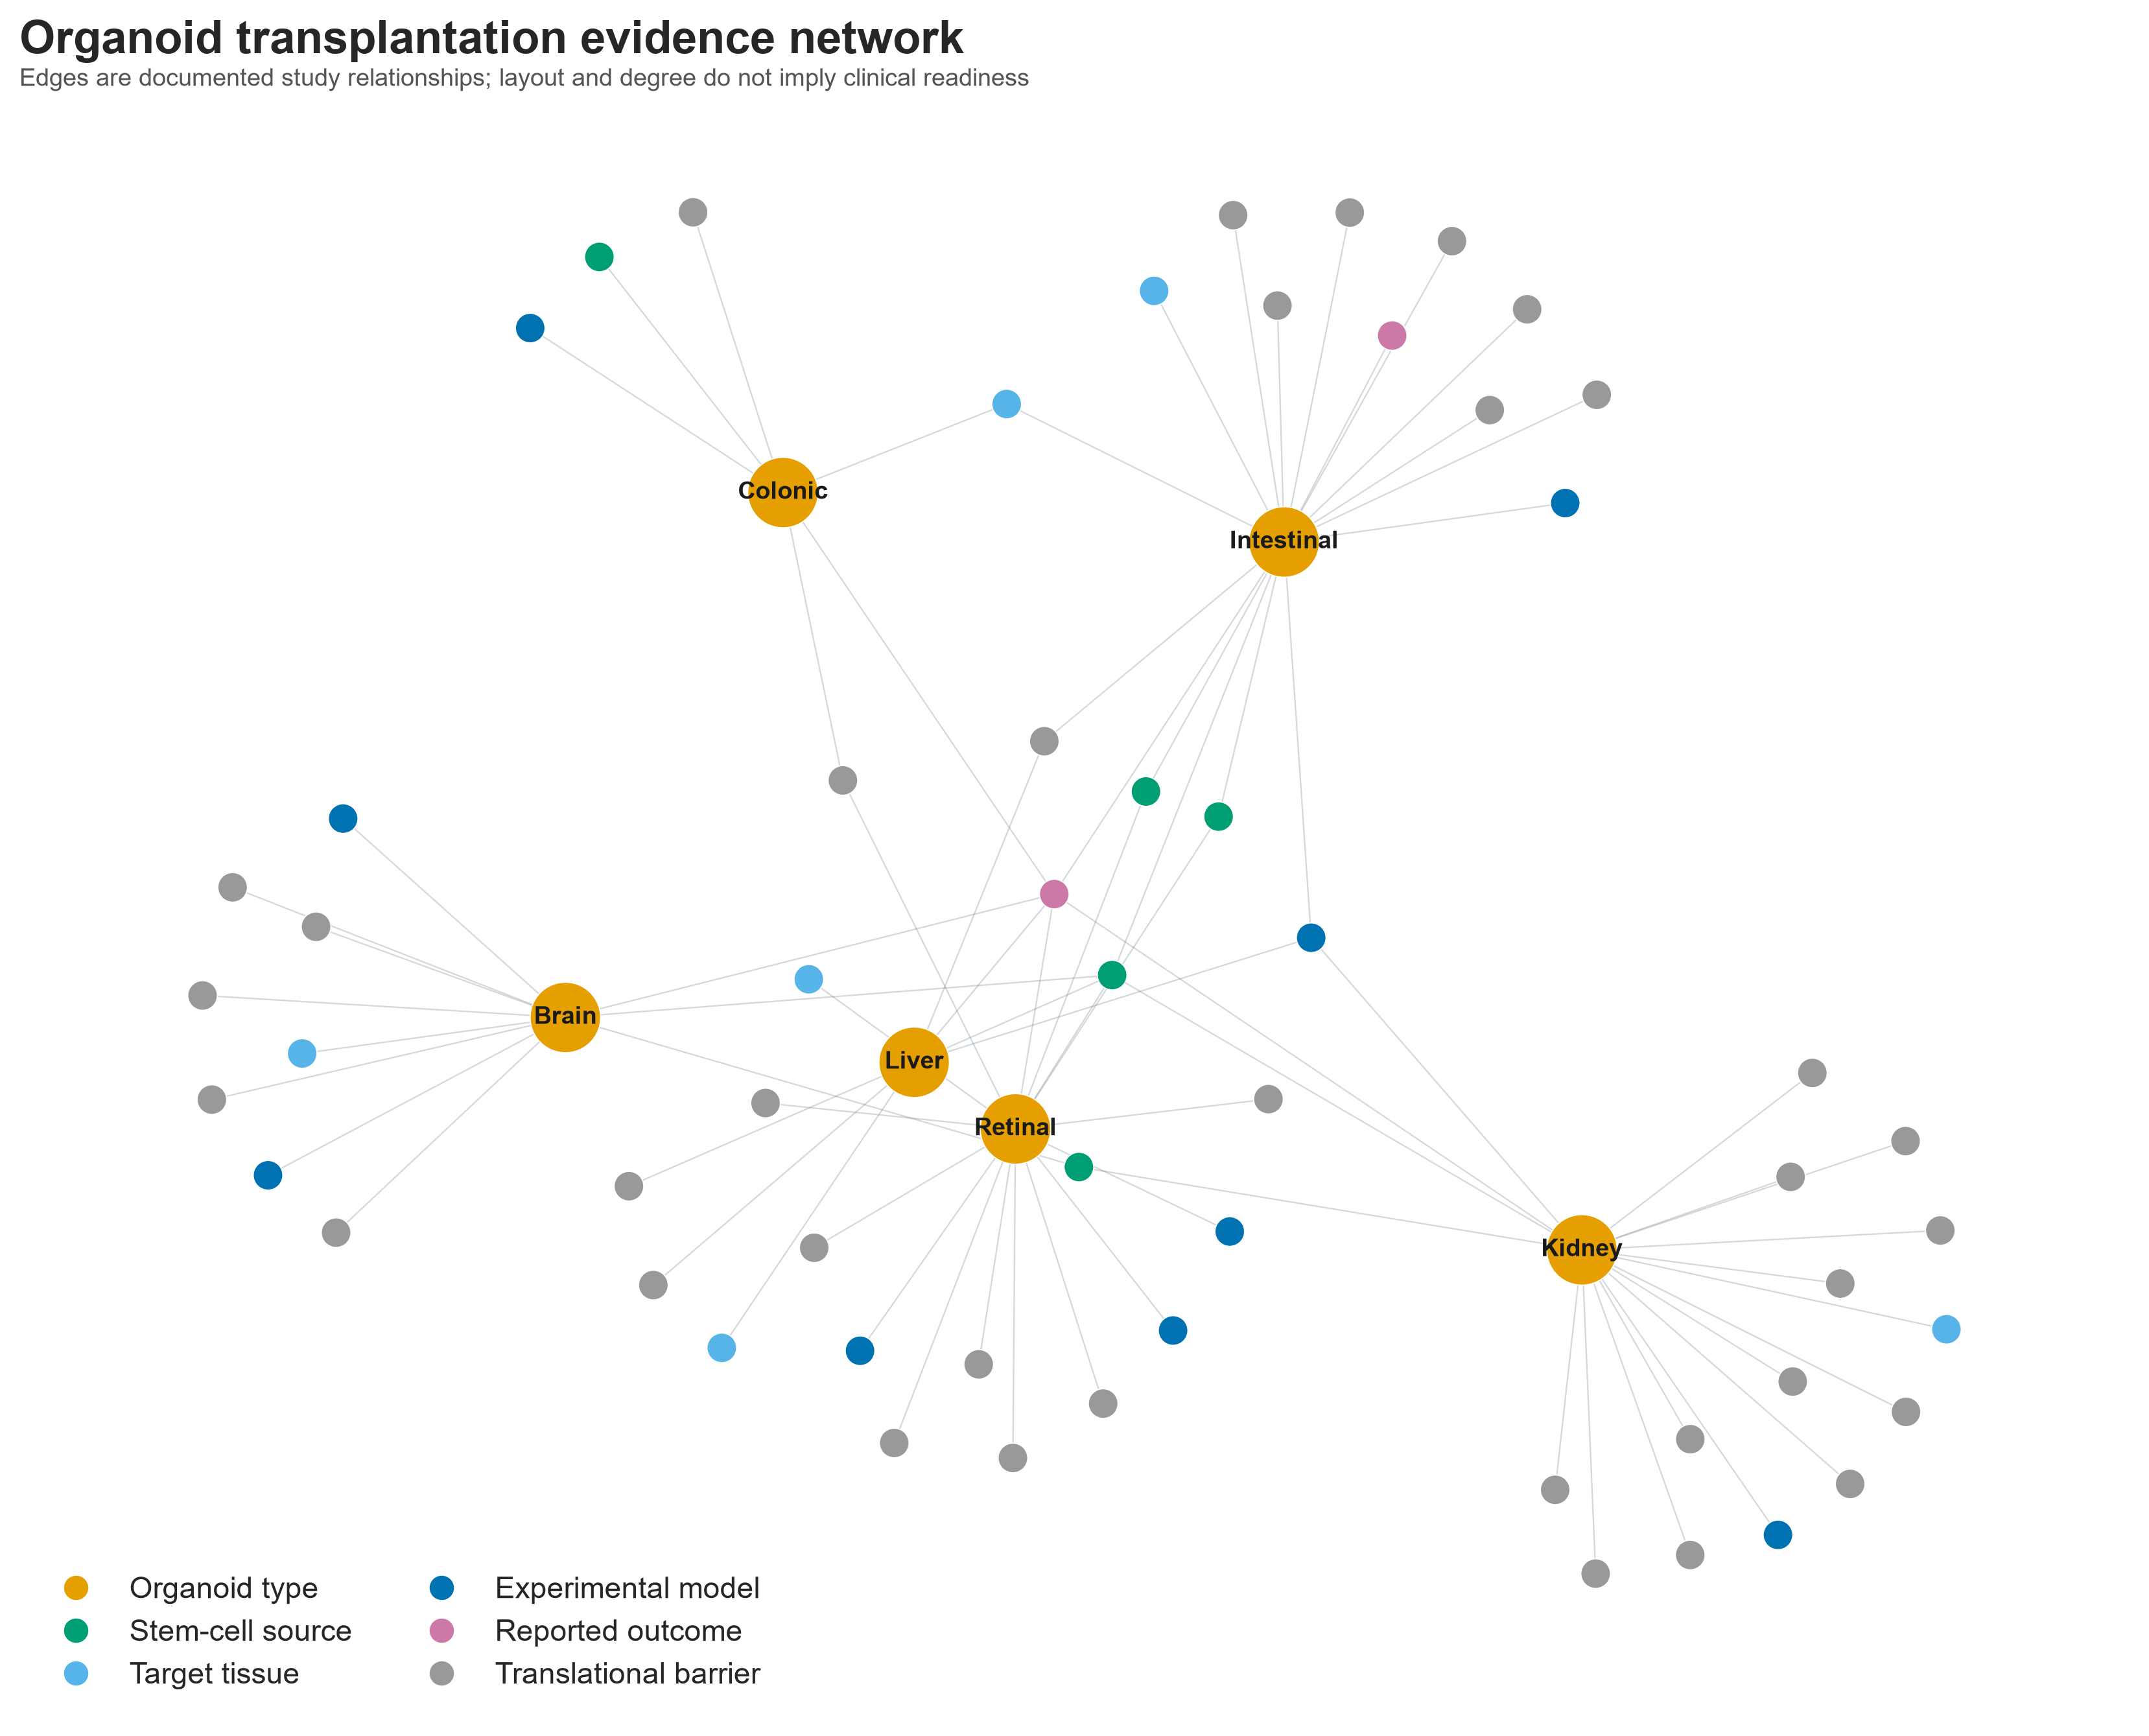
\includegraphics[width=\textwidth,height=0.73\textheight,keepaspectratio]{figure_05_research_network.png}
\caption{Evidence-backed organoid transplantation research network. Colour denotes node type, and each edge retains the IDs of studies that support the relationship. Network position and centrality describe the encoded literature structure; they do not measure treatment efficacy or clinical readiness.}
\label{fig:network}
\end{figure}

The graph is connected because common concepts---especially pluripotent-cell sources, animal models, positive engraftment states and recurring translational barriers---link the organoid categories. This connectedness is useful for finding shared design problems, but it is not evidence of biological interchangeability. A barrier node connected to several tissues may reflect repeated reporting or broad relevance; it does not quantify the severity of that barrier.

\subsection{Translational evidence matrix}

The matrix shows broad support for preclinical engraftment and functional maturation across the six organoid categories (Figure~\ref{fig:matrix}). Human clinical investigation is unassessed for every category in this corpus. Safety assessment is supported only for intestinal and retinal categories, while manufacturing and scale-up are largely unassessed or uncertain.

\begin{figure}[H]
\centering
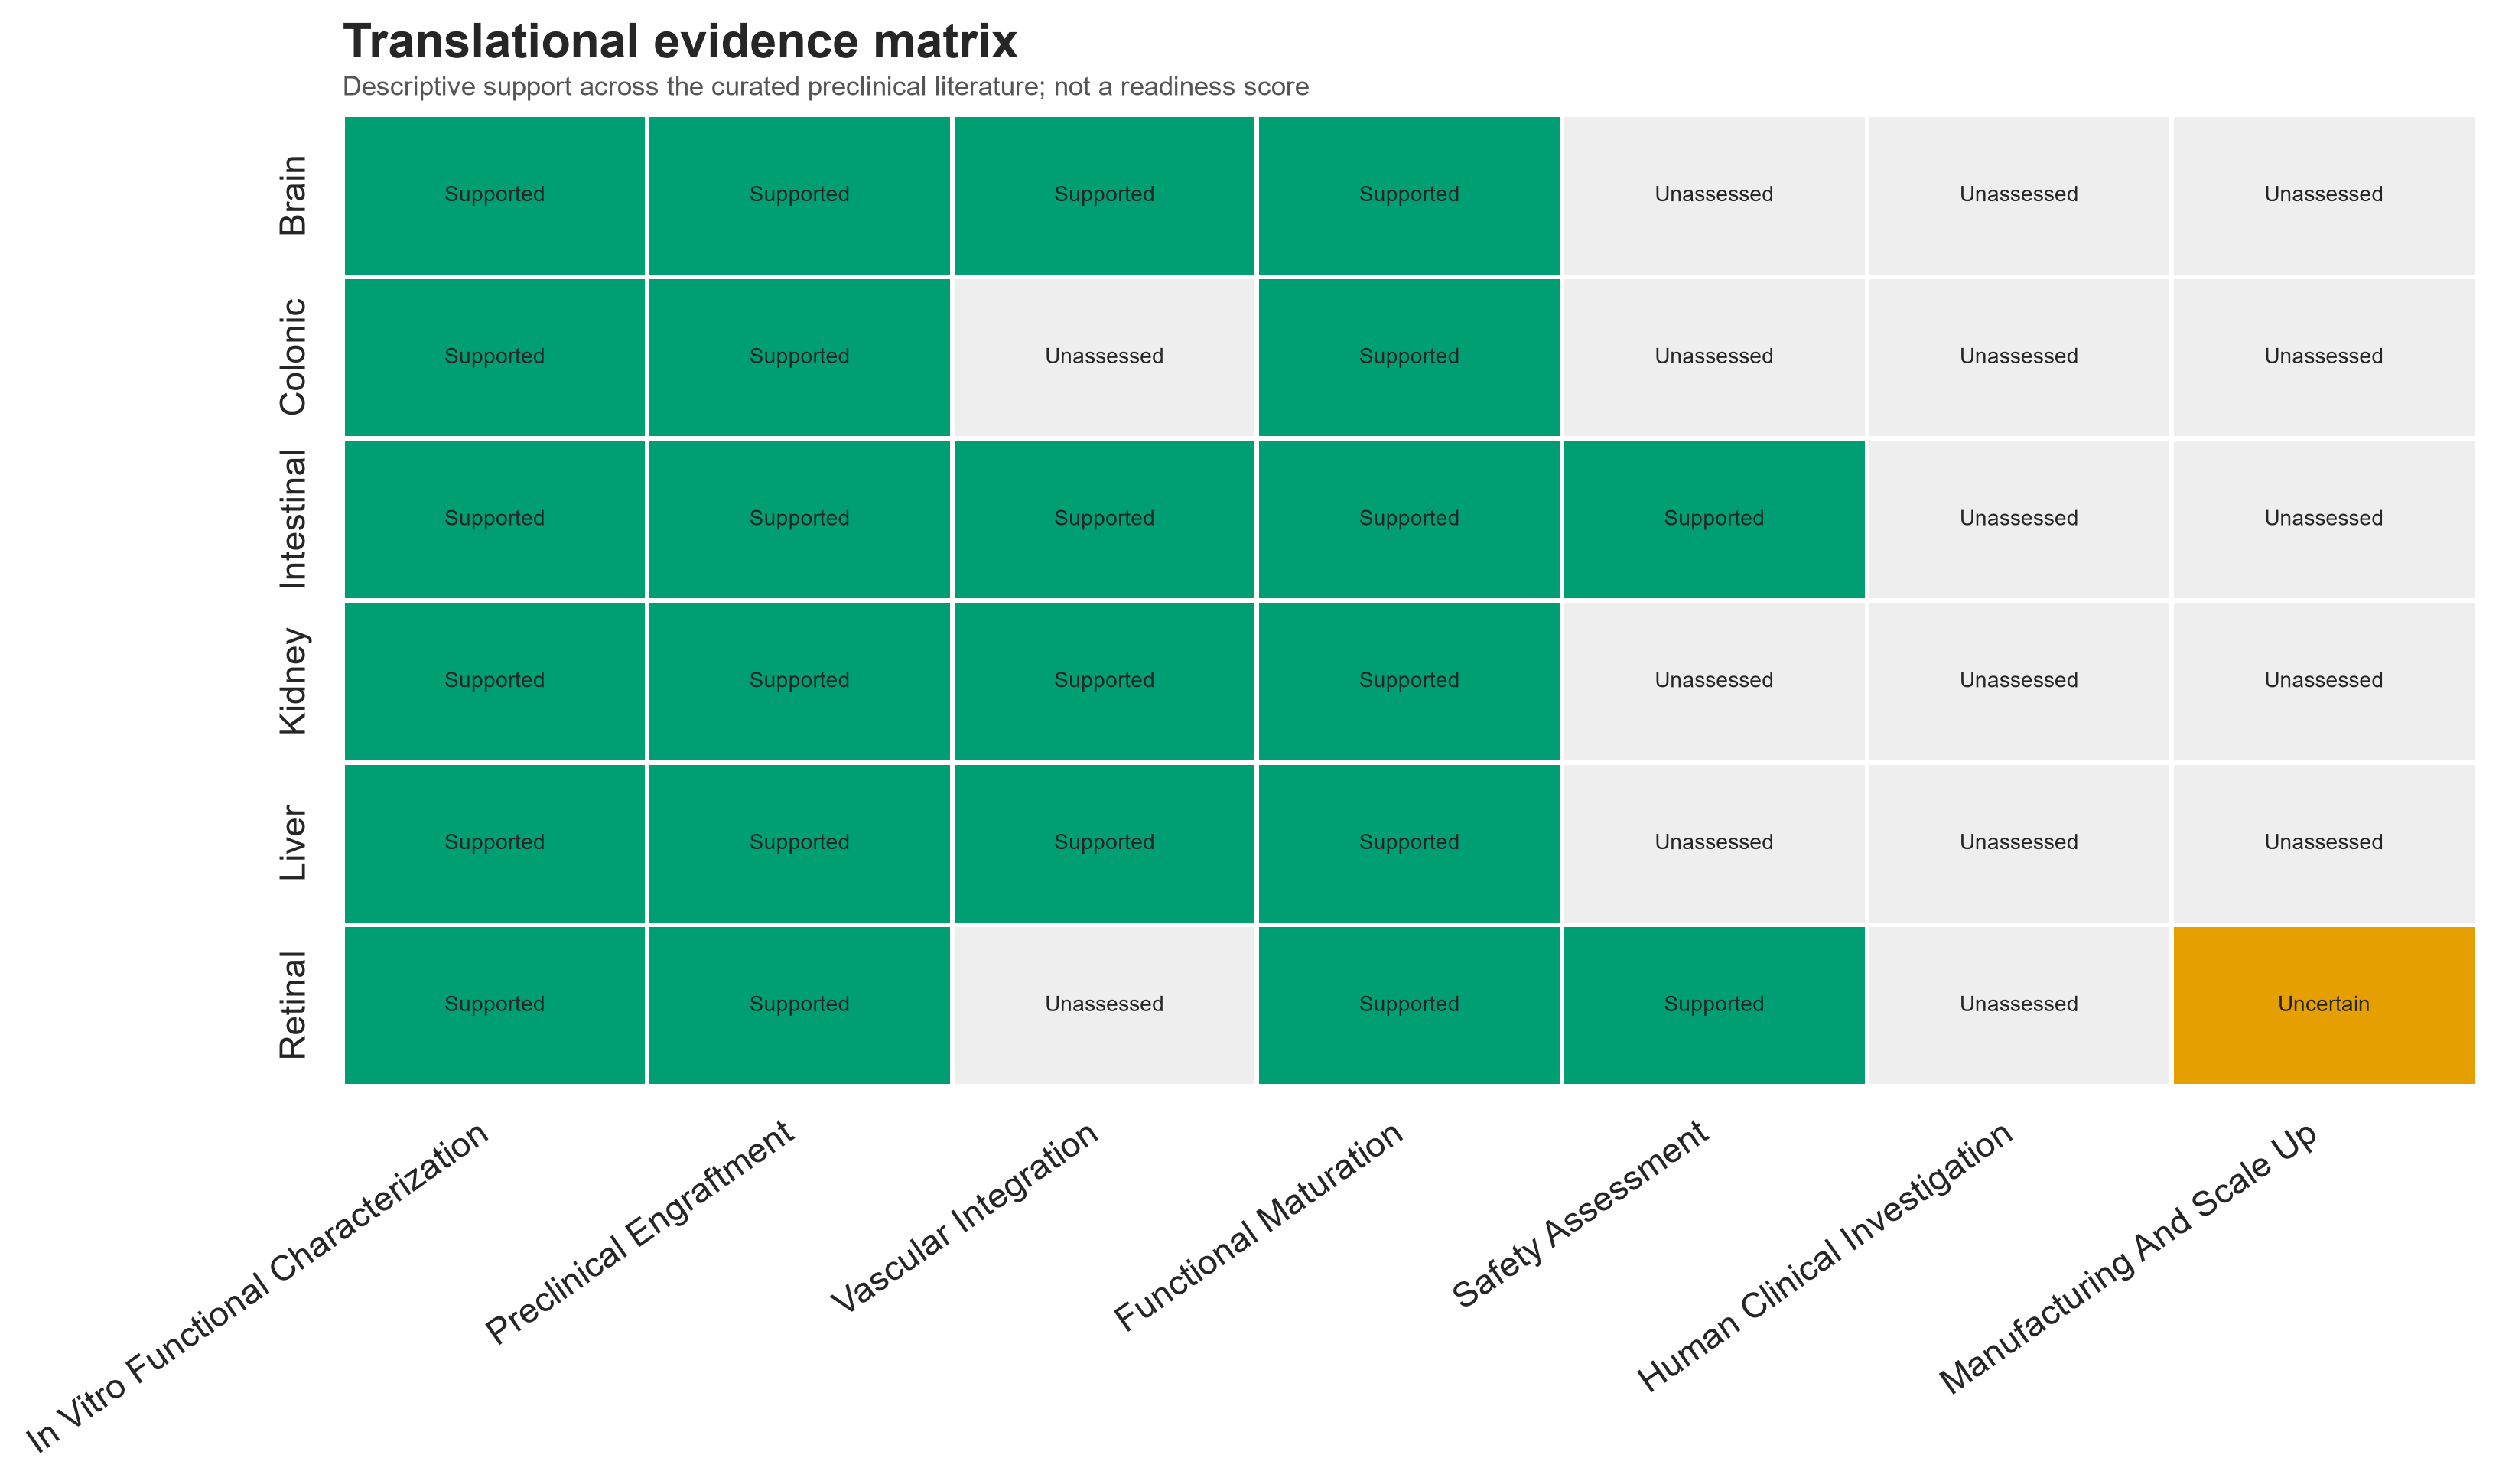
\includegraphics[width=\textwidth,height=0.55\textheight,keepaspectratio]{figure_06_translational_evidence_heatmap.png}
\caption{Translational evidence matrix. Cells summarize whether a domain is supported, unsupported, uncertain or unassessed within the bounded dataset. The display is descriptive and is not a clinical-readiness score.}
\label{fig:matrix}
\end{figure}

\begin{table}[H]
\centering
\small
\caption{Interpretive summary of the translational evidence matrix.}
\label{tab:matrixsummary}
\begin{tabularx}{\textwidth}{@{}P{22mm}YYY@{}}
\toprule
\textbf{Category} & \textbf{Stronger evidence in this corpus} & \textbf{Important unresolved domains} & \textbf{Interpretive boundary}\\
\midrule
Brain & Engraftment, vascularization, maturation and host-circuit interaction & Safety, manufacturing, immune effects and human investigation & Neural integration is not synonymous with therapeutic benefit\\
Colonic & Target-site epithelial engraftment and renewal & Vascular assessment, prospective safety and manufacture & Local epithelial repair does not replace full bowel physiology\\
Intestinal & Engraftment, vascularization and maturation at selected sites & Durable target-site repair, scale-up and human outcomes & Ectopic maturation must be separated from lesion repair\\
Kidney & Perfusion, nephron maturation and selected filtration features & Urinary drainage, nephron mass, long-term safety and human evidence & Microstructural filtration does not equal renal replacement\\
Liver & Vascular connection and partial metabolic function & Biliary integration, organ-scale reserve, safety and manufacture & Small ectopic graft function is partial physiology\\
Retinal & Sheet survival, maturation, functional signals and selected safety controls & Surgical consistency, off-target tissue, long-term function and scale-up & Animal visual responses require cautious clinical extrapolation\\
\bottomrule
\end{tabularx}
\end{table}

\subsection{Translational barriers and evidence gaps}

Recurring barriers include immature cell states, insufficient organ scale, vascular and immune compatibility, absent drainage or anatomical connection, inconsistent product identity and limited long-term safety evidence (Figure~\ref{fig:barriers}). The relative frequency of a barrier in the database records how often it was encoded, not its absolute importance.

\begin{figure}[H]
\centering
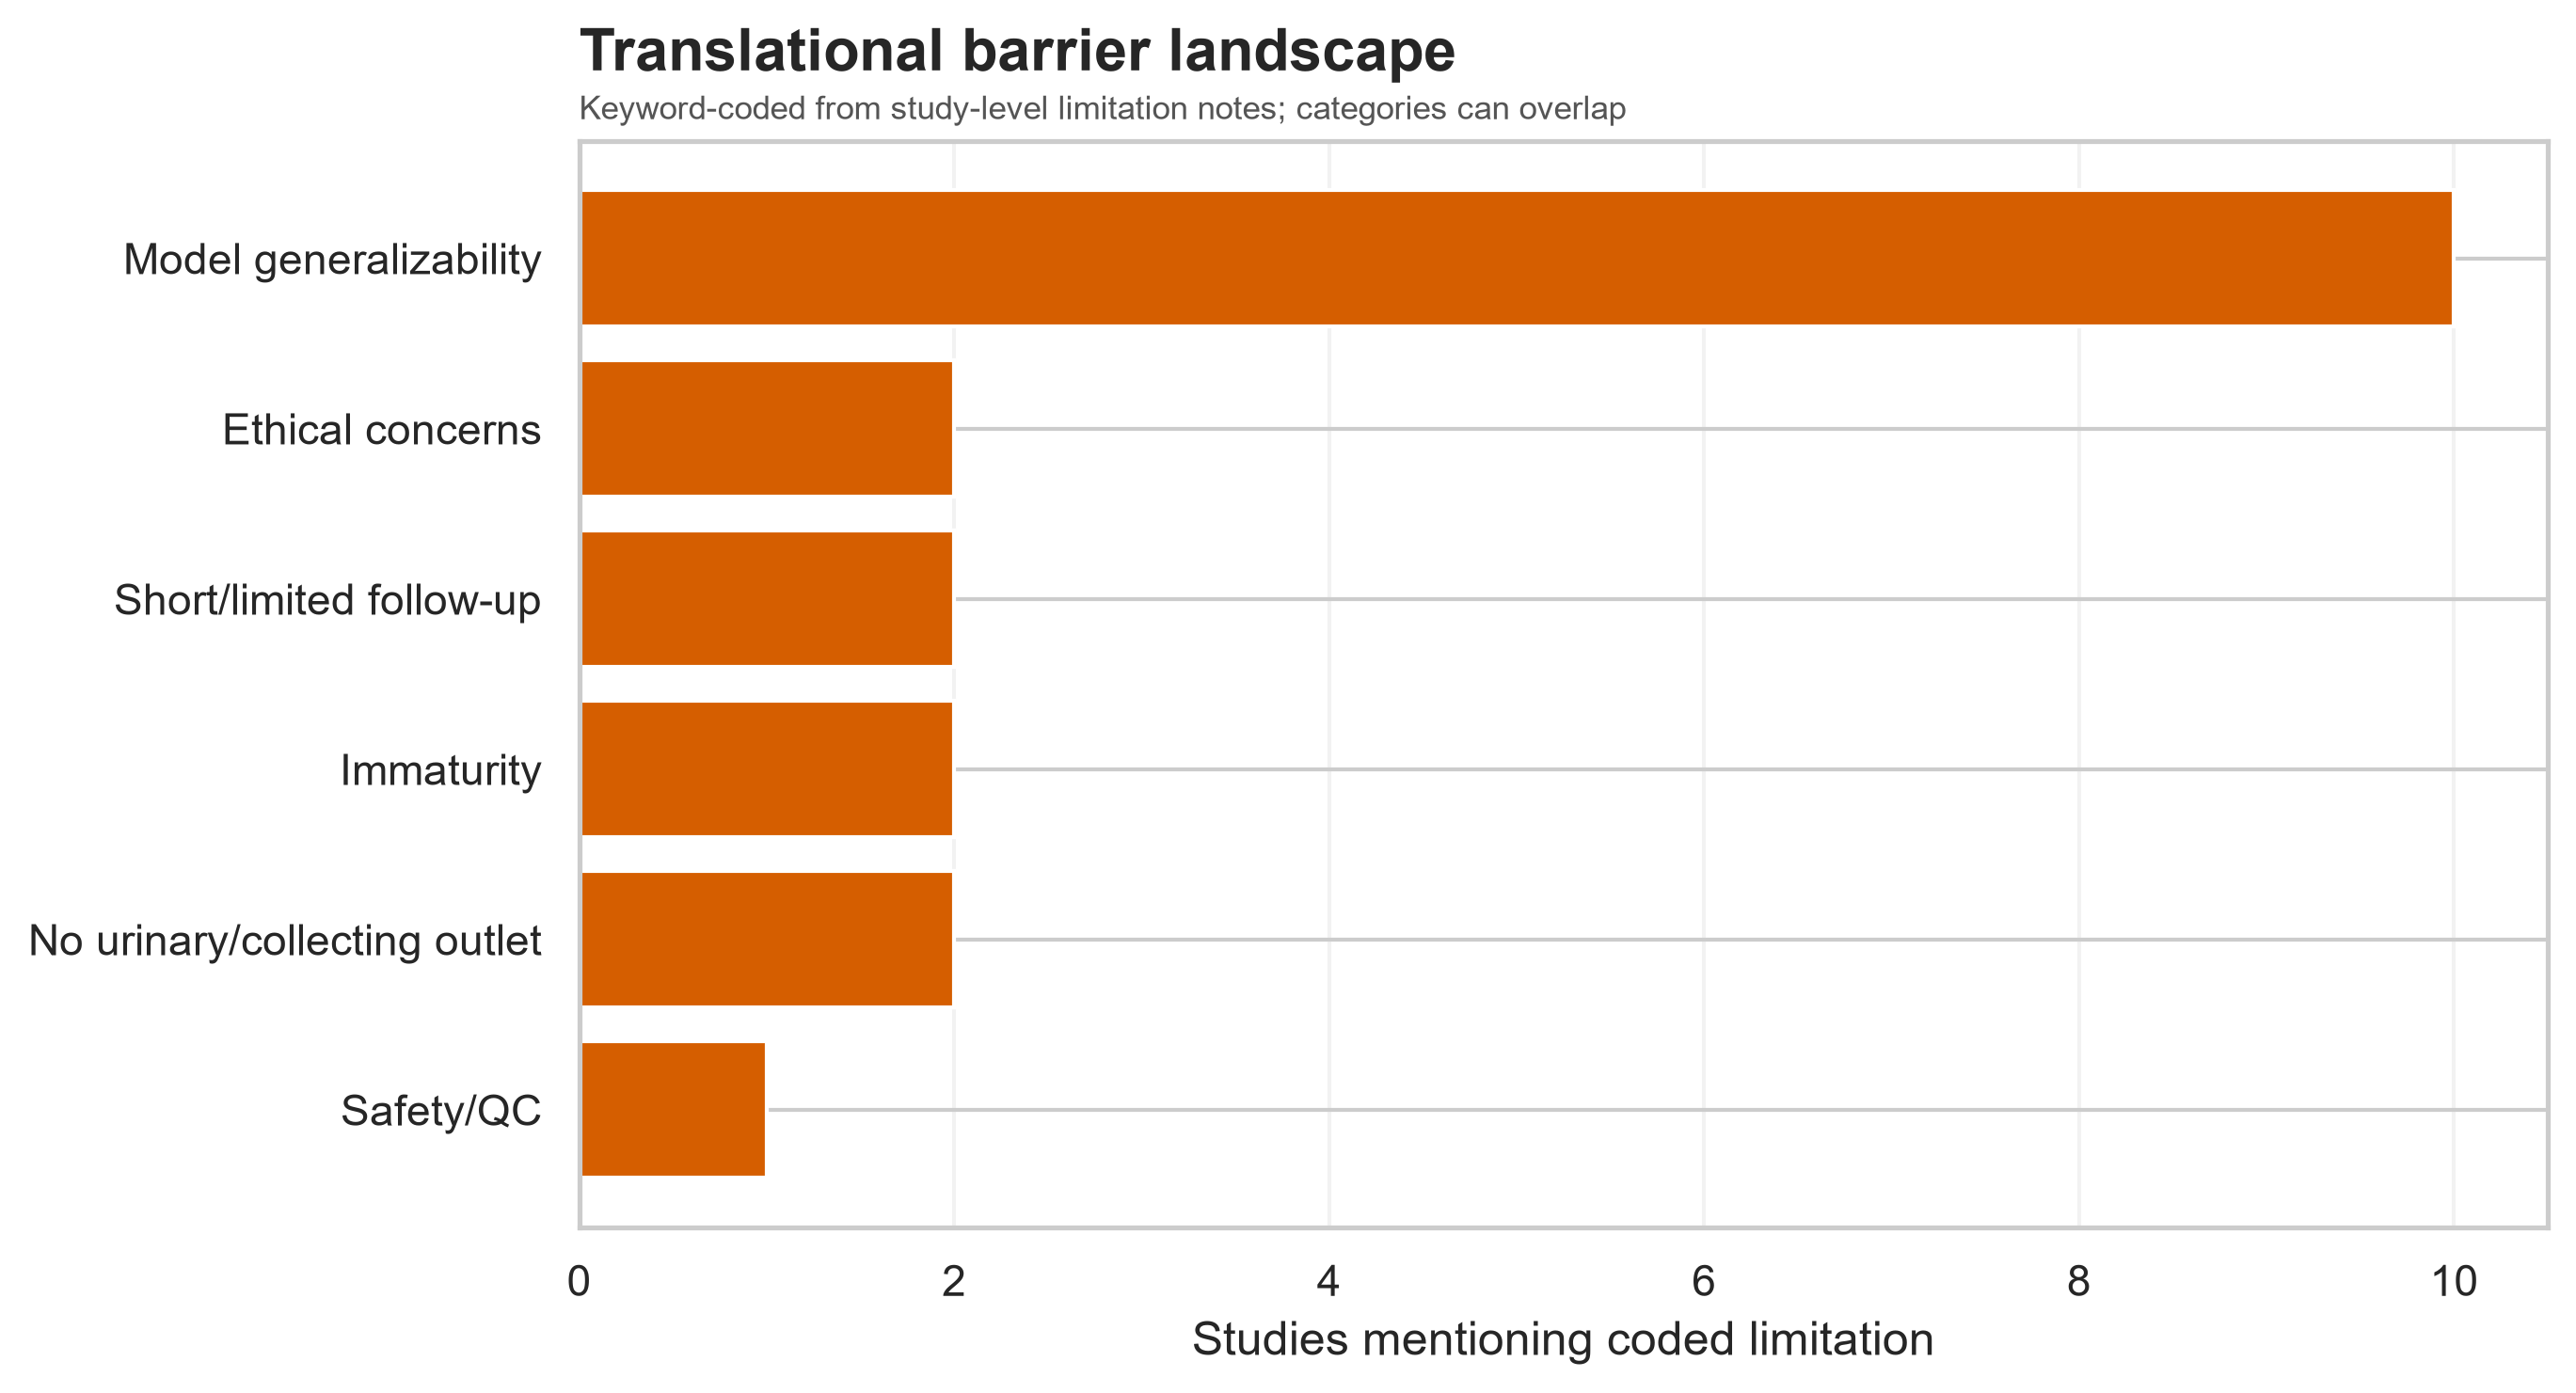
\includegraphics[width=0.94\textwidth]{figure_07_translational_barriers.png}
\caption{Documented translational barrier landscape. Counts derive from study-level limitations in the curated dataset and should be interpreted as reporting frequency within this corpus.}
\label{fig:barriers}
\end{figure}

Figure~\ref{fig:conceptual} places these barriers along a conceptual transplantation pathway. Quality control is required at each stage rather than only after grafting.

\begin{figure}[H]
\centering
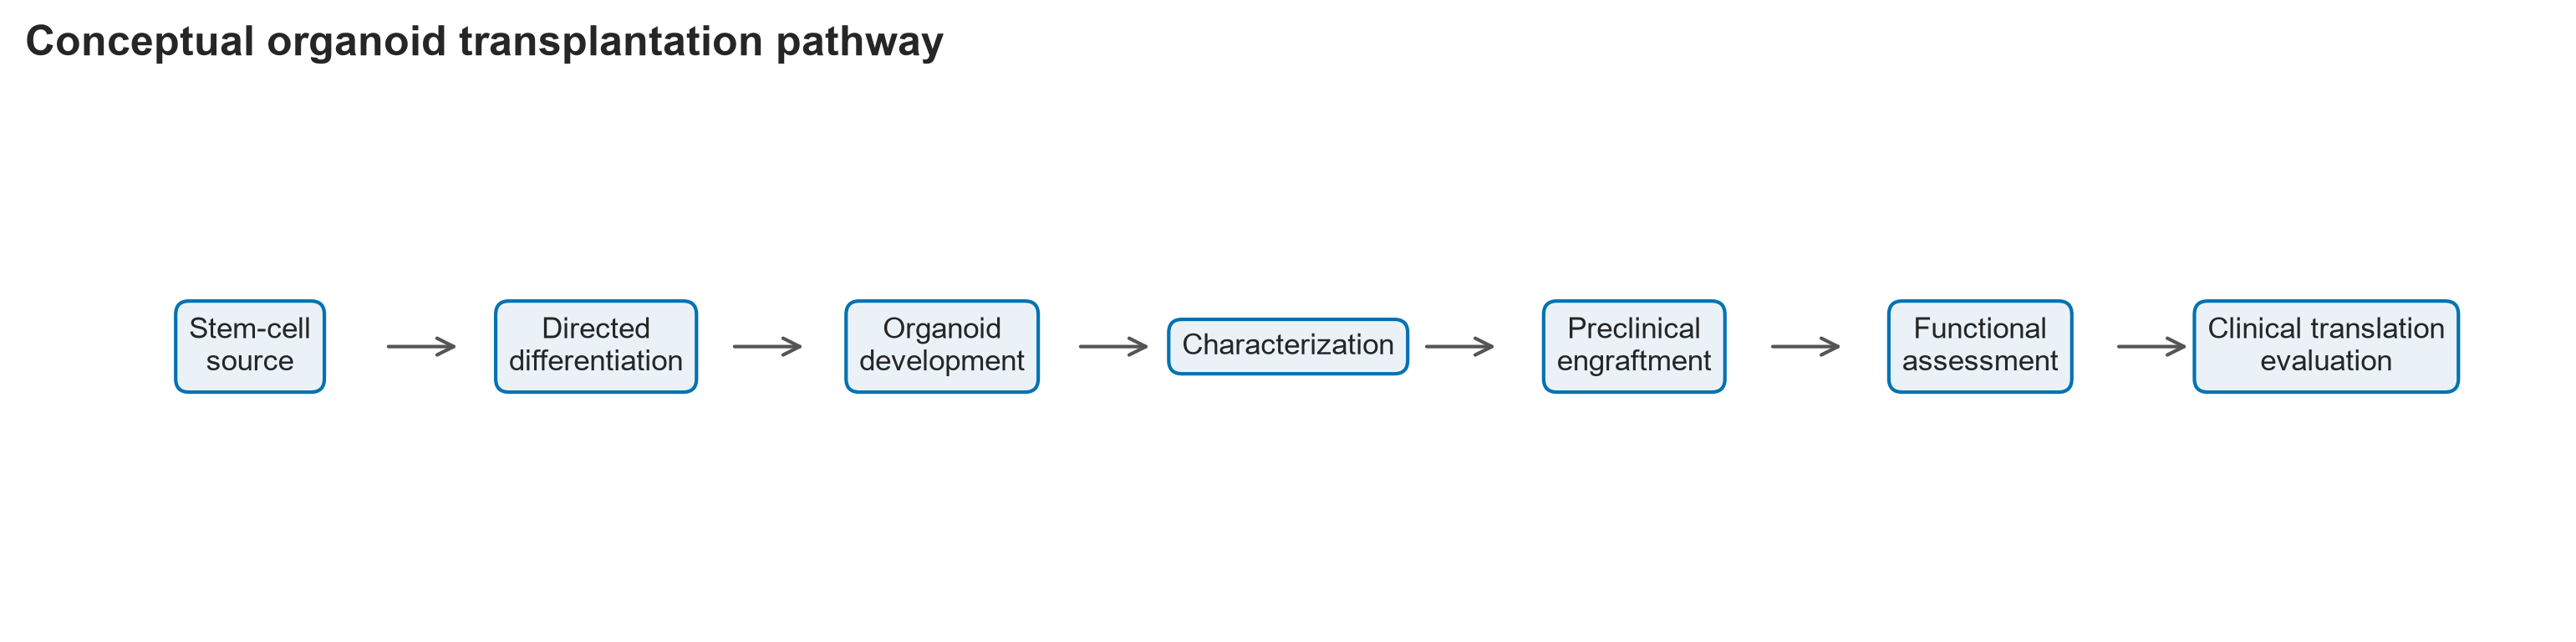
\includegraphics[width=0.97\textwidth]{figure_08_conceptual_transplantation_workflow.png}
\caption{Conceptual organoid transplantation pathway from cell source to translational evaluation. The diagram is an original synthesis and does not represent a single experimental protocol.}
\label{fig:conceptual}
\end{figure}

The most consequential evidence gaps occur after preclinical proof of concept: prospective safety, standardized manufacturing, immune compatibility, sustained physiological connection and human investigation (Figure~\ref{fig:gaps}). An unassessed cell indicates a gap in the mapped literature, not proof that the relevant biological capacity is absent.

\begin{figure}[H]
\centering
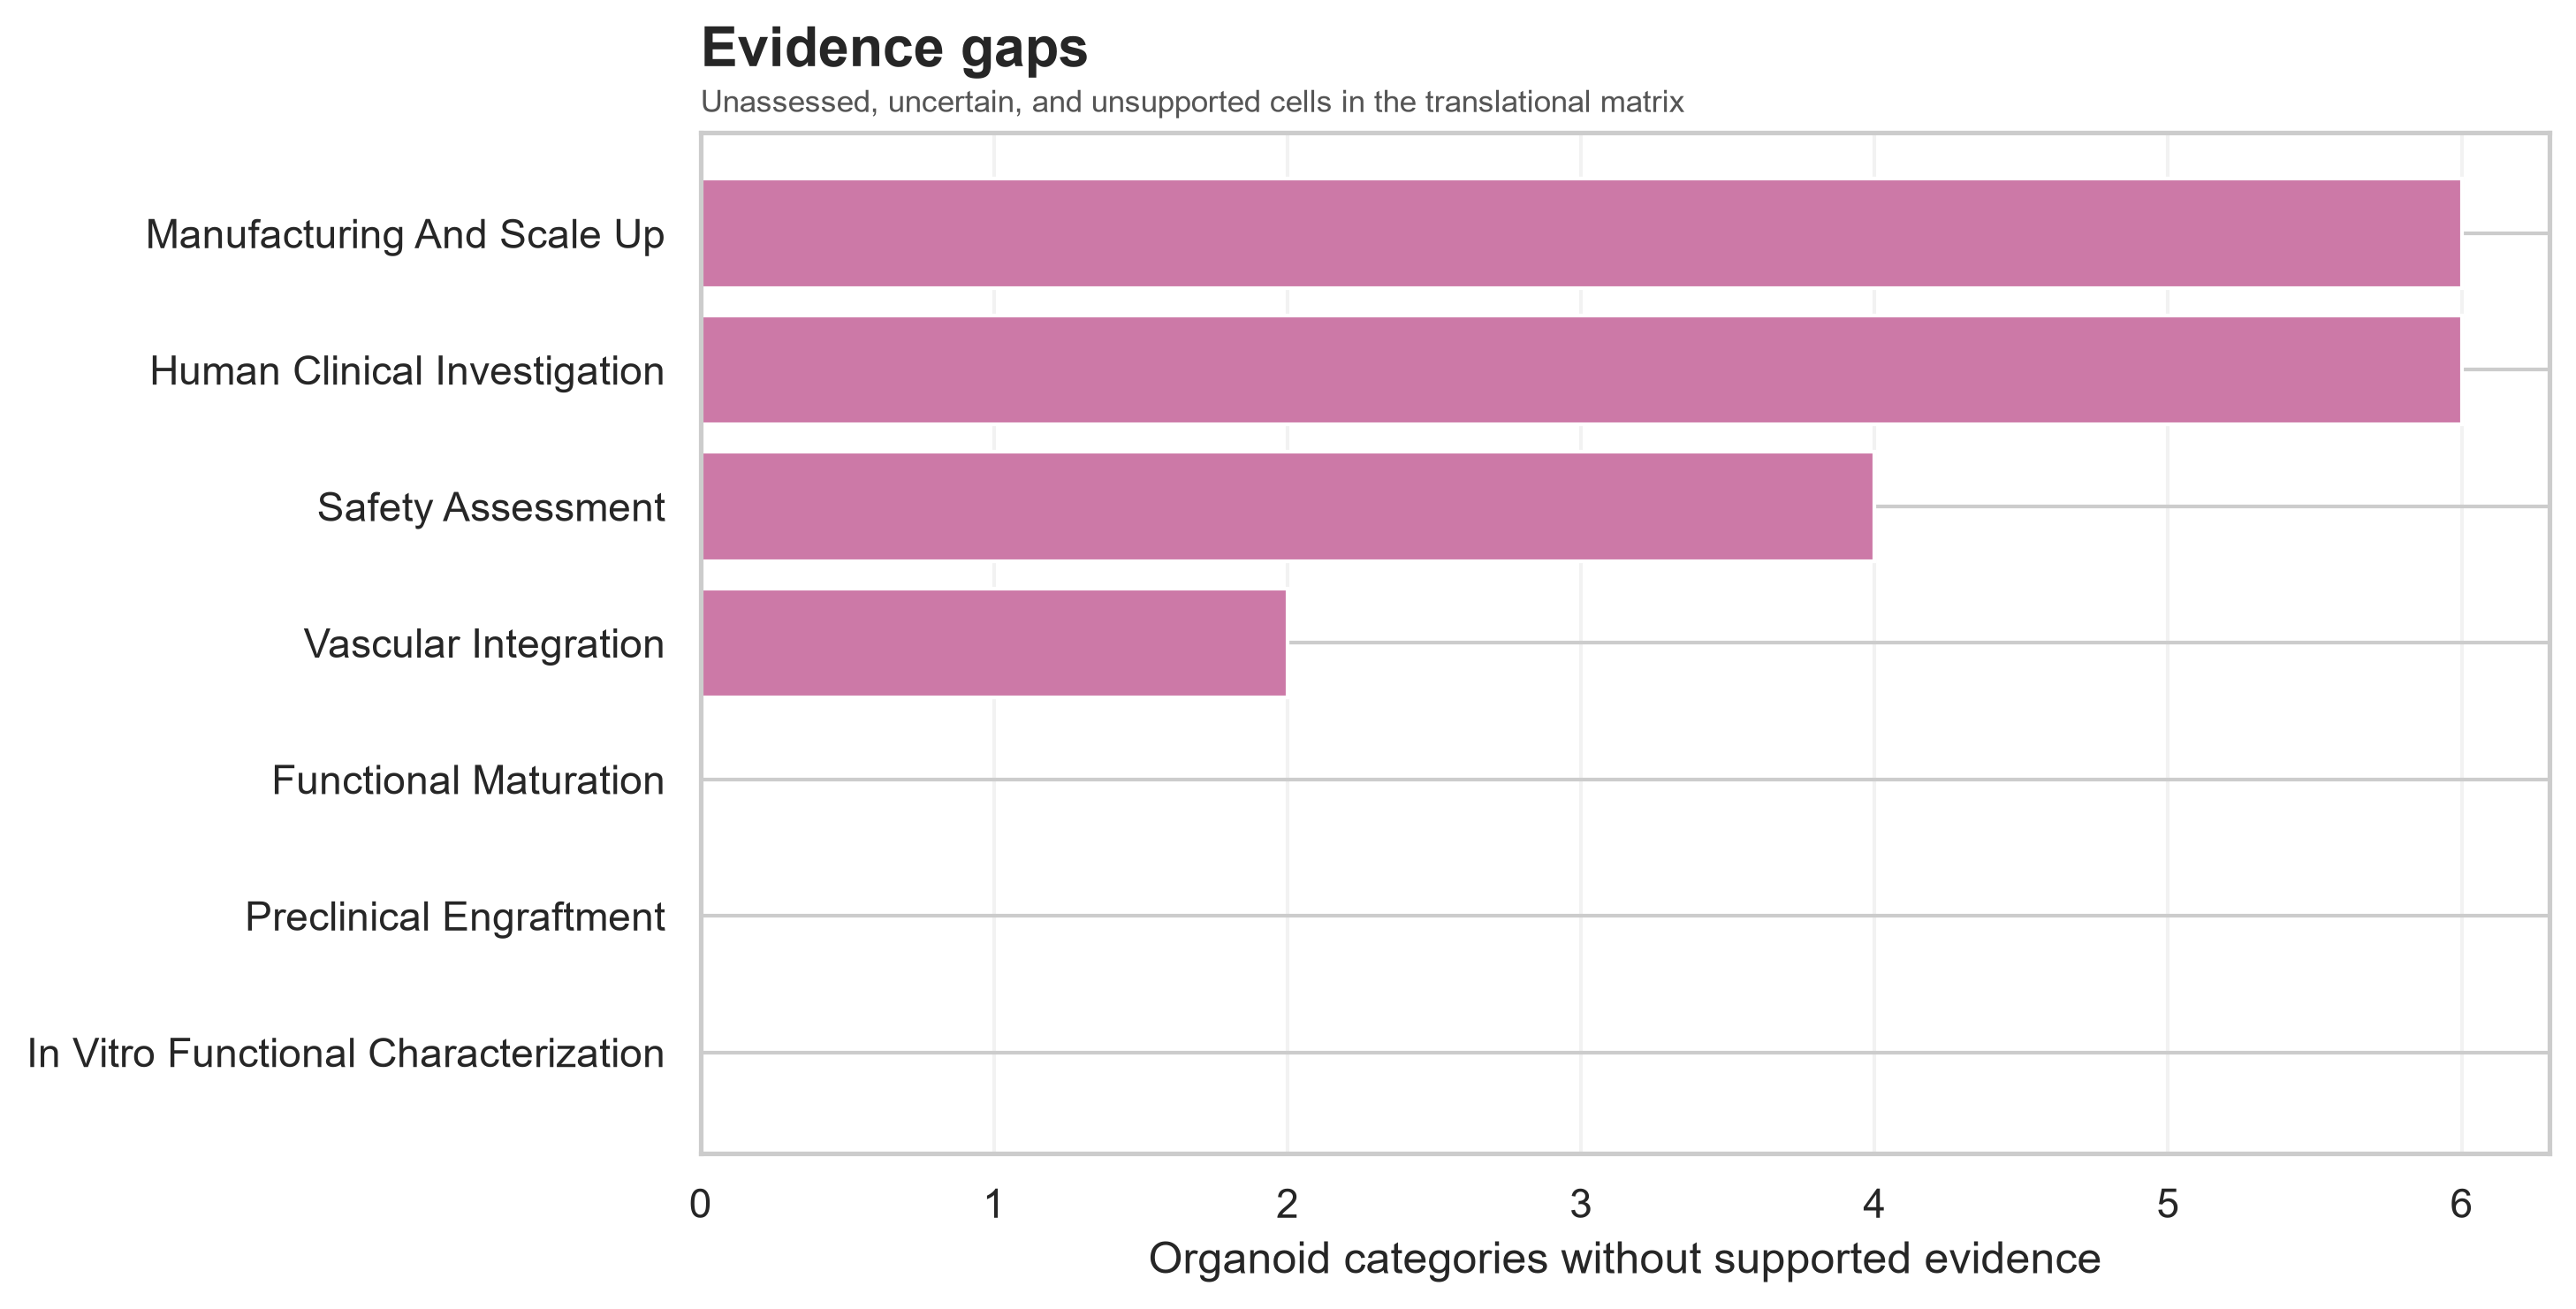
\includegraphics[width=0.94\textwidth]{figure_09_evidence_gaps.png}
\caption{Evidence-gap map derived from the translational matrix. Missing assessment is explicitly separated from negative evidence.}
\label{fig:gaps}
\end{figure}

\section{Discussion}

\subsection{Principal interpretation}

The mapped literature demonstrates that transplantation can expose organoid tissues to host-derived conditions that are difficult to recreate in static culture. Perfusion, extracellular matrix, systemic signalling and local injury cues can support survival and maturation. Across the included studies, these effects produced credible organ-specific observations, including epithelial renewal, vascularized tissue growth, nephron maturation, photoreceptor function and neural circuit interaction \citep{yui2012,takebe2013,watson2014,vandenberg2018,mclelland2018,revah2022}.

The same observations also show why translation requires restraint. Host support can obscure whether the graft itself contains a complete and controllable vascular programme. Ectopic implantation may maximize survival while avoiding the anatomical demands of the intended target. Immunodeficient recipients reduce rejection but provide limited information about immune compatibility. A short-lived physiological signal may be useful mechanistic evidence without demonstrating durable therapeutic function.

\subsection{Interpretation by tissue programme}

The intestinal and colonic evidence provides a useful contrast between maturation and repair. Human intestinal constructs can grow and mature after implantation, yet site selection determines whether the result is an ectopic tissue model or repair of a diseased bowel. The negative target-site result in ORG014 is therefore informative rather than contradictory: it defines a boundary condition that a purely positive-outcome narrative would miss.

Kidney research is the most represented programme in the corpus. Transplantation improves vascularization and maturation of glomerular and tubular compartments, and tracer experiments demonstrate selected filtration properties. Nevertheless, the absence of a connected collecting system and urinary outflow remains a decisive physiological limitation. Increasing the number of nephron-like structures without solving drainage, scale and endocrine integration would not yield a replacement kidney.

Retinal sheets and brain organoids demonstrate the value of tissue architecture. Organized retinal grafts can preserve cellular relationships relevant to photoreceptor replacement, while neural organoids can mature and participate in host circuits. Both applications require especially careful prospective safety evaluation. For retinal products, residual pluripotent or off-target tissue is a manufacturing concern. For neural grafts, unintended circuit effects and the ethical treatment of human--animal chimeric models require continuing oversight \citep{lovellbadge2021}.

The liver organ-bud study illustrates the strength and limitation of proof-of-concept biology. Rapid vascularization and measurable metabolic outputs show that multicellular organization can create function after grafting. Yet liver translation requires a much larger functional reserve, biliary architecture and durable integration. The result is best interpreted as an enabling demonstration rather than a near-clinical organ substitute.

\subsection{From experimental success to a transplantable product}

Moving from a laboratory construct to a clinical product requires a chain of linked controls:

\begin{enumerate}
  \item \textbf{Identity and purity:} defined cell composition, spatial organization and acceptable off-target populations;
  \item \textbf{Potency:} a validated assay connected to the intended mechanism of action;
  \item \textbf{Manufacturing consistency:} reproducible differentiation across lines, batches and facilities;
  \item \textbf{Delivery:} a graft format and surgical route compatible with the target anatomy;
  \item \textbf{Integration:} vascular, immune, neural or ductal connection appropriate to the organ;
  \item \textbf{Safety:} tumorigenicity, ectopic tissue, biodistribution, immunogenicity and long-term surveillance;
  \item \textbf{Clinical evidence:} prospective trials with endpoints that matter to patients.
\end{enumerate}

These requirements are consistent with the broader principle that stem-cell interventions should progress through rigorous, transparent and evidence-based clinical translation \citep{lovellbadge2021}. None can be inferred solely from a high engraftment frequency in animal studies.

\subsection{Manufacturing, biomaterials and immune translation}

The manufacturing problem begins before transplantation. Organoid phenotype depends on the starting cell line, passage history, differentiation timing, matrix composition, media lots and operator-dependent decisions. A clinically credible process therefore needs predefined critical quality attributes, acceptance ranges and in-process controls. Examples include cell identity and viability, lineage composition, spatial organization, genomic stability, residual pluripotency, sterility and a potency assay related to the intended mechanism \citep{rossi2018,hofer2021,jensen2023}. Automation can reduce handling variation, but it does not remove the need to justify which structural and functional features are essential.

Many research organoids are expanded in poorly defined or animal-derived extracellular matrices. Such matrices can be effective experimental substrates while remaining unsuitable as final clinical materials because composition, traceability and pathogen risk are difficult to control. Defined hydrogels, bioprinting, microfluidic perfusion and vascular co-culture provide routes toward reproducible geometry and improved mass transport, but each added component changes the product and its safety assessment \citep{brassard2019,park2024}. Scale-up should therefore preserve tissue quality rather than maximize cell number alone.

Autologous organoids may reduce some histocompatibility problems, but they require patient-specific manufacture, release testing and clinically practical timelines. Allogeneic products may be easier to standardize and bank, yet require attention to rejection, immunosuppression and donor-cell persistence. In either case, vascularization is not simply a matter of increasing capillary density: vessels must be stable, perfused and coordinated with organ-specific drainage or exchange. Reviews of personalized organoid medicine accordingly distinguish registered organoid-enabled studies from evidence that a transplantable organoid product has achieved clinical benefit \citep{sotogamez2024,septiana2024}.

\subsection{Priorities for the next generation of studies}

The evidence gaps suggest tissue-specific experiments rather than a universal next step (Table~\ref{tab:priorities}). The highest-value studies would combine mechanistic endpoints with prospective safety, explicit comparators and follow-up long enough to test durability.

\begin{table}[H]
\centering
\small
\caption{Tissue-specific research priorities derived from the mapped evidence and physiological requirements.}
\label{tab:priorities}
\begin{tabularx}{\textwidth}{@{}P{23mm}YYY@{}}
\toprule
\textbf{Programme} & \textbf{Critical experiment} & \textbf{Minimum outcome set} & \textbf{Key failure mode to exclude}\\
\midrule
Brain & Long-term, controlled graft studies in disease-relevant models & Cell fate, circuit activity, behaviour, host pathology and welfare & Unintended connectivity, overgrowth or misleading behavioural attribution\\
Colon/intestine & Orthotopic repair with barrier challenge and recurrence monitoring & Durable coverage, permeability, lineage renewal and inflammatory response & Ectopic growth or transient benefit without stable lesion repair\\
Kidney & Scaled constructs coupled to a collecting or drainage pathway & Perfusion, filtration, tubular transport, urine handling and endocrine markers & Perfused microstructures without useful excretory function\\
Liver & Larger grafts with biliary and metabolic integration & Synthetic function, detoxification, bile handling, perfusion and survival benefit & Partial biomarker production without adequate functional reserve\\
Retina & Standardized surgical delivery with masked functional assessment & Graft identity, visual physiology, behaviour, tumorigenicity and durability & Rosettes, off-target tissue, overgrowth or procedure-dependent bias\\
Cross-cutting & Multi-batch studies with predefined release criteria & Identity, potency, comparability, biodistribution, immunogenicity and safety & A favourable single batch that cannot be manufactured reproducibly\\
\bottomrule
\end{tabularx}
\end{table}

\subsection{Value of the computational evidence map}

The database, network and matrix serve different purposes. The database preserves study-level detail and source identifiers. The network reveals repeated relationships and shared barriers while retaining provenance on each edge. The matrix makes unassessed domains visible without falsely converting them to zero performance. Together, the three outputs provide a transparent basis for updating the corpus, checking claims and selecting future research priorities.

This approach also reduces two common interpretive errors. First, it prevents record counts from being reported as treatment effectiveness. Second, it prevents missing outcome reporting from being treated as a negative experimental result. These distinctions are essential in a young, heterogeneous field where studies often emphasize different biological questions.

\section{Limitations}

This evidence map has several important limitations. It is a single-reviewer, focused corpus rather than a database-complete systematic review. PubMed and backward citation checking were used, but formal searches of Embase, Web of Science, Scopus and grey literature were not completed. Dual independent screening and extraction were not performed. These constraints introduce selection and reviewer bias.

Some variables were extracted from bibliographic records and accessible report information rather than a harmonized full-text risk-of-bias assessment. Randomization, blinding, attrition, power calculations, exact sample sizes and follow-up durations require deeper study-level appraisal. The quality summary therefore reports identifiable domains and does not claim low risk of bias.

The corpus includes linked reports from related research programmes, so records are not necessarily independent experimental units. Species, immune status, disease model, graft location and outcome definition differ. Positive engraftment may refer to survival, structural integration or durable tissue replacement depending on the study. These differences preclude meta-analysis and make direct ranking inappropriate.

The absence of a human outcome report in this dataset applies only to the defined eligibility criteria and search date. It should not be interpreted as a timeless statement about every cell-based or organoid-related clinical activity. Likewise, an \emph{unassessed} matrix cell means that the mapped corpus did not evaluate the domain, not that the biological function is impossible.

\section{Conclusions}

Organoid transplantation has established credible preclinical proof of concept across intestinal, colonic, hepatic, renal, retinal and neural systems. Grafting can improve survival, perfusion and maturation and can produce tissue-specific functional signals. The evidence does not support treating these constructs as interchangeable therapies or as complete replacement organs.

The most persistent transition is from local animal-model function to a standardized, anatomically integrated and prospectively safe human product. Manufacturing control, immune compatibility, vascular and physiological connection, long-term safety and clinically meaningful outcome evidence remain central requirements. The computational framework developed here makes the present evidence traceable and updateable while keeping those uncertainties explicit.

\section{Data, code and reproducibility}

The repository contains the curated CSV dataset, data dictionary, provenance record, Python modules, six executed notebooks, GraphML network, translational matrix, nine PNG/SVG figure pairs, tests and release-validation utilities. The principal commands are:

\begin{verbatim}
python scripts/run_pipeline.py
python scripts/execute_notebooks.py
python -m pytest -v
python scripts/render_latex_report.py
python scripts/validate_release.py
\end{verbatim}

The completed validation used Python 3.14.2 with pinned project dependencies. The final software test run collected 11 tests; 11 passed, none failed and none were skipped. The graph contained 64 nodes and 75 edges, and every edge retained one or more valid supporting study IDs. Private source PDFs are not required to reproduce the computational outputs and remain excluded from the public repository.

\subsection*{Authorship and assistance disclosure}

Tharuniya Anpalakan is the author of this computational research project and remains responsible for the scientific interpretation, verification and any publication or reuse decision. OpenAI Codex materially assisted with software development, metadata checking, document preparation and language editing. It is not listed as a scientific author. This disclosure concerns the present computational project and does not alter the authorship of the earlier coauthored review \citep{sandamini2025}.

\subsection*{Citation note}

The bibliography uses Vancouver-style numbered citations in order of first appearance. It includes all 15 primary studies in the analytic corpus, foundational organoid-method studies, reporting guidance, major field reviews, a stem-cell translation guideline and the prior coauthored review. Background references inform interpretation but were not counted as eligible transplantation studies.

\clearpage
\bibliographystyle{vancouver}
\bibliography{../references/bibliography}

\end{document}
